\documentclass{article}
\usepackage[utf8]{inputenc}
\usepackage[english]{babel}
\usepackage[a4paper, total={7in, 9in}]{geometry}
\usepackage{graphicx}
\usepackage{float}
\usepackage{verbatim}
\usepackage[bottom]{footmisc}
\usepackage[style=numeric]{biblatex}
\usepackage{minted}
\usepackage{csquotes}
\usepackage{fancyvrb}
\usepackage[title]{appendix}
\usepackage{xcolor}
\addbibresource{references.bib}

\newcommand{\titleRule}{
    \rule{\linewidth}{0.5mm} \\ [0.25cm]
}

\begin{document}

{
\center
\textsc{\Large Universidade do Minho} \\ [0.5cm]
\textsc{\Large Mestrado Integrado em Engenharia Informática} \\ [0.5cm]
\textsc{\large Engenharia de Sistemas de Computação} \\ [0.5cm]

{\LARGE \bfseries Análise das NAS Parallel Benchmarks} \\[0.2cm]

\begin{tabular}{c c}
    José Carlos Lima Martins & Miguel Miranda Quaresma \\
    A78821 & A77049  \\
\end{tabular} \\[0.5cm]

\today \\[1cm]
}



\section{Introdução}

\quad O estudo do comportamento de sistemas de computação está frequentemente relacionado com o estudo da \textit{performance} do mesmos.
Este estudo recorre a um conjunto de métricas que se referem às diversas componentes dos sistema (disco, memória principal,
CPU, rede, etc) e que podem ser obtidas com recurso a algumas ferramentas disponibilizadas pelo próprio sistema.
O presente trabalho apresenta uma análise ao comportamento de um subconjunto das \textbf{N}AS \textbf{P}arallel \textit{\textbf{B}enchmarks} (NPB) e à forma como estas influenciam o sistema onde são executadas.

As NPB são um conjunto de \textit{benchmarks} desenvolvidas pela \textit{NASA Advanced Supercomputing Division} com o intuito de auxiliar a 
avaliação de performance de supercomputadores. Este conjunto é constituído por 5 \textit{kernels} (IS, EP, CG, MG e FT) e 3 pseudo-aplicações 
(BT, SP e LU).  Possui ainda 3 versões multi-zona (BT-MZ, SP-MZ e LU-MZ) que exploram múltiplos níveis de paralelismo, 4 \textit{benchmarks} 
para computação não estruturada (UA, BT-IO, DC e DT), bem como 4 \textit{benchmarks} para testar a performance de \textit{grids} computacionais 
(ED, HC, VP e MB). 

De entre esta gama de \textit{benchmarks} o presente trabalho utiliza duas: FT, \textit{discrete 3D fast Fourier Transform}, com comunicação todos 
para todos, e LU (\textit{Lower-Upper Gauss-Seidel solver}) versão multizone (LU-MZ), com zonas de igual tamanho dentro de uma classe do problema 
e um número fixo de zonas para todas as classes de problema.



\section{Metodologias de teste}

\quad O conjunto de \textit{benchmarks} que compreendem as NPB engloba \textit{benchmarks} de diversos tipos, sendo que para cada \textit{benchmark}
individual é ainda possível alterar a carga computacional através do parâmetro \textit{CLASS}.
O presente trabalho estuda as classes A e B das \textit{benchmarks} anteriormente referidas.

Os testes realizados com as duas \textit{benchmarks} alteram diversos parâmetros entre testes dos quais se destacam: 
\begin{itemize}
    \item nodos utilizados
        \begin{itemize}
            \item r641
            \item r431
        \end{itemize}
    \item compiladores usados
        \begin{itemize}
            \item Intel (versão 19.0.0.117)
            \item GNU (versão 5.3.0)
        \end{itemize}
    \item \textit{flags} de compilação utilizadas 
        \begin{itemize}
            \item \texttt{-O2}
            \item \texttt{-O3}
            \item \texttt{-Ofast} (\textit{fast math, less accuracy})
        \end{itemize}
    \item tecnologias de comunicação
        \begin{itemize}
            \item \textit{Ethernet}
            %\item \textit{Myrinet} (nodo r641)
        \end{itemize}
\end{itemize}

É importante realçar que a realização de testes em dois nodos diferentes permite testar as \textit{benchmarks} em micro-arquiteturas 
de processadores distintas, \textit{Nehalem} (nodo r431) e \textit{Ivy Bridge} (nodo r641) no caso dos nodos referidos.

Dadas as \textit{benchmarks} realizadas possuírem implementações de memória distribuída que recorrem à biblioteca OpenMPI, foi usada a versão
1.8.2 da mesma, tanto na implementação da GNU como na implementação da Intel.

É importante também referir que a implementação OpenMP para a \textit{benchmark} FT foi executada com 32 \textit{threads} para o nodo r641 
(16 \textit{cores} físicos, 32 \textit{cores} lógicos) e 24 \textit{threads} para o r431 (12 \textit{cores} físicos, 24 \textit{cores} lógicos).

A implementação OpenMP da \textit{benchmark} LU-MZ foi testada com 16 \textit{threads} visto que o número de zonas do algoritmo é 16, o que limita o número 
de \textit{threads}/processos a 16 \cite{lumzLimitProcs}. Para a classe B desta \textit{benchmark} foi necessário, previamente à sua execução, definir as 
seguintes variáveis de ambiente:
\begin{verbatim}
export OMP_STACKSIZE=500m //OMP
export KMP_STACKSIZE=500m //Intel
export GOMP_STACKSIZE=500m //GNU
\end{verbatim}
por forma a haver espaço suficiente de alocação.

A implementação MPI de ambas as \textit{benchmarks} foi testada em dois nodos r641 (ou r431) e 8 processos.


\subsection{Dados e Ferramentas}

\quad Como foi referido anteriormente, a análise da \textit{performance} de sistemas recorre a ferramentas disponibilizadas pelo sistema que 
permitem estudar diversos componentes do mesmo.
Considerando como componentes de relevo o CPU, a memória principal, a utilização de rede e as operações de I/O, apresentam-se de seguida
as métricas recolhidas e as ferramentas usadas para as recolher: 
\begin{itemize}
    \item \textbf{utilização de CPU}: \texttt{pidstat -u <sample\_rate>}
    \item \textbf{ocupação de memória}: \texttt{vmstat 1}
    \item \textbf{utilização da memória}: \texttt{pidstat -r <sample\_rate>} e \texttt{sar -r <sample\_rate>}
    \item \textbf{utilização de disco baseada no tempo}: \texttt{iostat -d 1} e \texttt{vmstat -d 1}
    \item \textbf{utilização da rede}: \texttt{sar -r <sample\_rate> -n DEV} (estatísticas da rede)
    \item \textbf{saturação da rede}: \texttt{sar -r <sample\_rate> -n EDEV} (estatísticas de erro)
\end{itemize}

Esta análise faz parte da primeira fase do \textit{USE Method} em que se pretende tentar localizar a(s) zona(s) de erro analisando a \textbf{U}tilização, 
\textbf{S}aturação e \textbf{E}rros para, posteriormente, realizar uma análise mais especifica nessa(s) zona(s) identificada(s) como provocadora(s) de 
problemas/perda de \textit{performance}.

A realização dos diversos casos de teste referidos foi automatizada com recurso a \textit{scripts bash} (FT: \ref{FTscript}) para cada \textit{benchmark} 
que alterassem os parâmetros automaticamente, e registassem os dados obtidos através das ferramentas referidas, gravando-os em ficheiros de texto.



\section{Análise dos resultados}

\quad A análise de resultados apresentada consistirá na comparação dos dados obtidos nos diferentes testes por forma a permitir compreender
o comportamento das \textit{benchmarks} e a forma como estas condicionam o sistema em que foram testadas, consoante os parâmetros definidos para as mesmas.
Adicionalmente, e consoante a natureza das comparações efetuadas, \textbf{i.e.} quais os parâmetros em que estas diferem (\textbf{e.g.} 
\textit{flags} de compilação utilizadas), serão omitidas certas métricas dado não sofrerem variações ou não serem afetadas pelos parâmetros
alterados.


\subsection{SER vs. OMP vs. MPI}

\quad As \textit{benchmarks} NAS apresentam duas implementações paralelas que diferem no paradigma utilizado (memória partilhada/OpenMP e memória
distribuída/OpenMPI) e uma implementação sequencial. Dadas as características de cada uma destas implementações torna-se útil comparar o comportamento
de cada implementação bem como o seu impacto no sistema.

A utilização do disco no tempo foi considerada desprezável na presente comparação dado que o disco se trata de um recurso partilhado por diversos nodos
do \textit{cluster} e, como tal, a sua utilização não depende apenas das \textit{benchmarks} em questão, variando consoante o tipo e a dimensão da carga 
que outros utilizadores coloquem no sistema.


\subsubsection{\textit{Benchmark} FT}

\quad A observação dos gráficos (ver \ref{fig:ft_ser_omp_mpi_r641_intel}, \ref{fig:ft_ser_omp_mpi_r641_gnu}) com os resultados obtidos nas três 
implementações da \textit{benchmark} FT: SER (sequencial), OMP (memória partilhada) e MPI (memória distribuída) permite identificar diferenças em 
diversas métricas.
Uma diferença considerável está presente na utilização (baseada na capacidade) do CPU que é consideravelmente superior na implementação OMP, sendo
a sua mediana igual a 2962.14\% no nodo r641 e 2302.5\% no nodo r431. Esta diferença é justificada pelo facto da implementação OMP recorrer a fios de 
execução (\textit{threads}) que são escalonados no CPU e que, com recurso à capacidade de \textit{hyperthreading}, permite que mais que uma \textit{thread}
esteja em execução num dado instante no mesmo CPU.
Adicionalmente, é possível observar que a utilização de memória da implementação MPI é consideravelmente superior do que as restantes, que se deve
ao facto de a mesma envolver a criação de processos que replicam o espaço de memória do processo "pai", resultando numa maior utilização da memória
devido à redundância inerente a este mecanismo.

Por fim, é possível observar que a comunicação inerente a implementações em memória distribuída com processos comunicantes leva a que a implementação 
MPI resulte numa maior utilização da rede, no número de pacotes recebidos e transferidos (\texttt{rxpck/s} e \texttt{txpck/s}), algo que não se verifica
nas restantes implementações.


\subsubsection{\textit{Benchmark} LU-MZ}

A observação dos gráficos (ver \ref{fig:lumz_ser_omp_mpi_r641_intel}, \ref{fig:lumz_ser_omp_mpi_r641_gnu}) que contêm as métricas mais relevantes para a
comparação das implementações SER, OMP e MPI desta \textit{benchmark} (LU-MZ) permite, num instante inicial, verificar que, tal como na \textit{benchmark} FT, 
a implementação OMP apresenta uma utilização de CPU (\texttt{\%CPU}) 12-15x superior às restantes implementações, que se deve à capacidade de 
\textit{hyperthreading} dos processadores que permite que mais que uma \textit{thread} esteja em execução num dado \textit{core} no mesmo instante, resultando 
numa utilização superior a 100\%. 
Adicionalmente, o consumo de memória é consideravelmente superior no caso da implementação MPI, justificado pelo facto de esta se tratar de uma implementação num 
paradigma de memória distribuída (com processos comunicantes) em que a criação de processos envolve a cópia da memória do processo com \textit{rank} 0, 
resultando num maior consumo de memória. Por outro lado, é ainda importante realçar o aumento considerável na utilização da rede, mais concretamente no 
número de pacotes recebidos (\texttt{rxpck/s}) e transmitidos (\texttt{rxpck/s}) pelo nodo motivado pela comunicação inter-processo inerente ao paradigma 
de memória distribuída.


\subsection{Comparação entre classes: A vs. B}

\quad As diferentes classes disponibilizadas pelas \textit{benchmarks} NAS diferem na dimensão dos \textit{datasets} utilizados nos 
testes, resultando em diferentes cargas colocadas no sistema em que estas são executadas. O presente trabalho envolveu testes com 
as classes A e B, cujas características para cada uma das \textit{benchmarks} serão de seguida apresentadas.


\subsubsection{Benchmark FT}

\quad A carga computacional da \textit{benchmark} FT varia em função do número de iterações do algoritmo e no tamanho da grelha sobre 
a qual este trabalha, sendo estes os parâmetros afetados pelas classes. No caso das classes A e B, o número de iterações não se altera, 
sendo igual a 20, ao invés do tamanho da grelha que passa de 256 x 256 x 128  para 512 x 256 x 256. Um dos impacto óbvios 
(ver \ref{fig:ft_A_B_r641_intel} e \ref{fig:ft_A_B_r431_intel}) desta alteração prende-se com o consumo de memória \textbf{i.e.} a sua 
utilização face à capacidade da mesma. Por outro lado, um aumento do número de dados resulta num aumento direto do tempo de computação, 
consequência direta da complexidade computacional deste algoritmo ($O(N log N )$ \cite{fft_complexity}), que leva a que, apesar do uso 
baseado em capacidade do CPU não se altere, o seu uso baseado no tempo seja superior.


\subsubsection{Benchmark LU-MZ}

\quad A diferença entre as classes A e B para a \textit{benchmark} LU em versão multi-zona reflete-se no tamanho da grelha utilizada, 
que passa de 128 x 128 x 16 para 304 x 208 x 17 que, consequentemente, se reflete nos requisitos de memória da \textit{benchmark} que, 
segundo a especificação, são de 50MB para a classe A e 200MB para a classe B.

Estes diferenças (ver \ref{fig:lumz_A_B_r641_intel} e \ref{fig:lumz_A_B_r431_intel}) refletem-se na utilização de memória registada 
pelos dados obtidos. Por outro lado, através da análise do output de cada uma das \textit{benchmarks}, é também possível identificar 
diferenças no tempo de execução que permitem concluir que, ainda que não sejam registadas variações significativas na utilização, 
baseada na capacidade, do CPU e da memória, a sua utilização baseada no tempo será superior dado que o tempo de execução, como foi 
referido, será superior.


\subsection{Comparação entre compiladores: GNU vs. Intel}

\quad O impacto de diferentes compiladores no comportamento de uma dada aplicação está relacionado com o código \textit{Assembly} gerado
pelos mesmos, que diferem entre compiladores. Estas diferenças podem resultar em ganhos (ou perdas) de \textit{performance}. Adicionalmente,
determinadas diferenças podem ser introduzidas com o uso de \textit{flags} de compilação, dado que estas introduzem otimizações  que diferem
consoante o compilador e a \textit{flag} usados. 


\subsubsection{\textit{Benchmark} FT}

\quad Na implementação MPI é possível constatar, pelos gráficos \ref{fig:ft_gnu_intel_r641} e \ref{fig:ft_gnu_intel_r431}, algumas diferenças entre 
os compiladores GNU e Intel, tanto na utilização de CPU como de memória, que são inferiores (cerca de metade) na versão compilada com Intel face à 
compilada com GNU. Para além disso, na implementação OMP visualiza-se que a utilização de CPU é superior com o compilador da GNU quando comparada com
a gerada pelo compilador da Intel, visto a versão compilada pela Intel ser mais otimizada para o \textit{hardware} utilizado, aproveitando melhor (de forma mais eficiente) as caraterísticas
do mesmo. Por fim, verifica-se que a implementação OMP apresenta uma utilização de CPU (\textit{\%CPU}) maior pela simples razão de possuir mais 
processos/\textit{threads} que as outras versões (Sequencial e MPI). 


\subsubsection{\textit{Benchmark} LU-MZ}

\quad A visualização dos gráficos \ref{fig:lumz_gnu_intel_r641} e \ref{fig:lumz_gnu_intel_r431} não permite identificar diferenças significativas entre
os dois compiladores, tanto na utilização de memória como de CPU. Contudo, é possível observar que na implementação OMP as versões geradas com o 
compilador GNU resultam numa utilização de CPU superior às geradas com o compilador Intel. 


\subsection{Comparação entre nodos/\textit{hardware}: r641 vs. r431}

\quad A execução de testes em máquinas com diferentes características de hardware, nomeadamente na micro-arquitetura do processador e 
quantidade de memória RAM, pode resultar num comportamento diferente do sistema visto que, por exemplo, micro-arquiteturas mais recentes 
possuem otimizações ao nível do escalonamento de instruções ou no número de unidades funcionais que permitem obter maior \textit{performance} em
aplicações que explorem este tipo de paralelismo (ILP). Tendo estes fatores em conta, a comparação efetuada considera os parâmetros referentes à
utilização de CPU e de memória, bem como da rede.


\subsubsection{\textit{Benchmark} FT}

\quad A observação do gráfico \ref{fig:FT_r641_r431} permite concluir que a diferença mais significativa entre os dois nodos diz respeito à utilização de CPU. 
Os dados recolhidos permitem observar que, na implementação OMP, a utilização de CPU é consideravelmente superior no nodo r641, algo que pode ser justificado
pelo facto deste nodo possuir um processador com uma micro-arquitetura mais recente levando a que o mesmo seja mais eficiente no escalonamento de \textit{threads}
maximizando, por isso, a utilização do CPU. Por outro lado, o facto das máquinas diferirem no número de \textit{cores} leva a que a sua capacidade de executar
\textit{threads} em paralelo seja diferente, sendo menor no caso do nodo r431 que possui apenas 12 \textit{cores} ao invés do nodo r641 que possui 16 \textit{cores}.
Adicionalmente é possível observar diferenças na utilização de memória (\texttt{\%memused}) que é consideravelmente superior no nodo r431, derivado do
facto da sua memória principal ser apenas de 12/48GB ao invés do nodo r641 que possui uma memória principal com 64GB.


\subsubsection{\textit{Benchmark} LU-MZ}

\quad A observação do gráfico \ref{fig:LUMZ_r641_r431} permite identificar diversas diferenças no comportamento dos nodos para o mesmo teste. Uma das 
principais diferenças entre os dois nodos, no que diz respeito à utilização de CPU, prende-se com a percentagem desta utilização que é passada a executar 
código em \textit{user space}, que é superior no nodo r431. Isto pode ser justificado pelo facto deste nodo possuir um processador com uma micro-arquitetura
anterior à do nodo r641 que, como foi referido anteriormente, apresenta uma \textit{performance} inferior que resulta num aumento no tempo de execução. 
Ainda na utilização de CPU é possível identificar uma diferença significativa no comportamento das implementações OMP em ambos os nodos que, como 
foi referido, pode ser justificada pelas diferentes micro-arquiteturas dos processadores envolvidos. Adicionalmente é ainda possível verificar que a utilização de memória, baseada na capacidade, é superior no nodo r431. Como esta métrica é relativa à capacidade da memória (64GB no caso do nodo r641; 12 ou 48GB 
no caso do nodo r431) este resultado corresponde ao que seria esperado, dado que a mesma quantidade de memória representará uma percentagem superior 
no nodo r431. É ainda importante realçar que, nos testes da implementação OMP com compilador GNU e otimização \texttt{-O3}, esta diferença é menos notória, devido à 
existência de nodos do tipo r431 com uma quantidade de memória mais próxima da do nodo r641.


\subsection{Comparação entre \textit{benchmarks}: FT vs. LU-MZ}

\quad A execução de algoritmos distintos condiciona consideravelmente o comportamento de uma determinada aplicação e, consequentemente da forma 
como esta condiciona o sistema em que é executada. Isto deve-se ao facto de algoritmos distintos envolverem não só operações diferentes mas 
também a manipulação de estruturas de dados distintas, alterando, por exemplo, a quantidade de operações que envolvem comunicação de dados ou 
a quantidade de memória necessária para armazenar as estruturas de dados. A observação dos gráficos \ref{fig:FT_LUMZ_r641} e \ref{fig:FT_LUMZ_r431} 
permite visualizar a diferença entre a utilização de memória da \textit{benchmark} FT e da \textit{benchmark} LU-MZ, que é consideravelmente superior 
na primeira, chegando a tomar valores próximos do dobro da segunda para o mesmo teste (\textbf{e.g.} a versão sequencial de FT consome 2.385 de 
\texttt{\%MEM} por comparação com 1.25\% da versão sequencial de LU-MZ, ambas geradas com o compilador Intel e \textit{flag} \texttt{-O3}).
Atentando aos valores referente à comunicação e, mais concretamente, aos valores referentes à quantidade de pacotes transmitidos e recebidos por segundo, 
\texttt{rxpck/s} e  \texttt{txpck/s} respetivamente, é também possível observar que, para o mesmo teste, a utilização da rede por parte da 
\textit{benchmark} FT é bastante superior à da LU-MZ. No entanto, é importante realçar que isto não resulta numa saturação da rede, não 
podendo ser considerado como possível causa para problemas na \textit{performance} do sistema.

\section{Conclusão}
\quad A análise dos resultados anteriores permite concluir que a \textit{benchmark} FT apresenta um melhor aproveitamento dos recursos disponíveis 
face à \textit{benchmark} LU-MZ. 
Adicionalmente, os valores obtidos referentes à utilização do disco não permitiram inferir conclusões concretas quanto ao comportamento do sistema
dado que este recurso (disco) é partilhado por diversos nodos do \textit{cluster}. A análise efetuada permitiu ainda observar que as implementações 
MPI das \textit{benchmarks} apresentam uma utilização da rede superior pela simples razão de serem desenvolvidos num paradigma de memória distribuída 
com processos comunicantes em execução em nodos distintos.

\printbibliography

\newpage 
\begin{appendices}
\section{Resultados Obtidos}

\subsection{Benchmark FT}

\subsubsection{Nodo r641}

\begin{figure}[H]
    \centering
    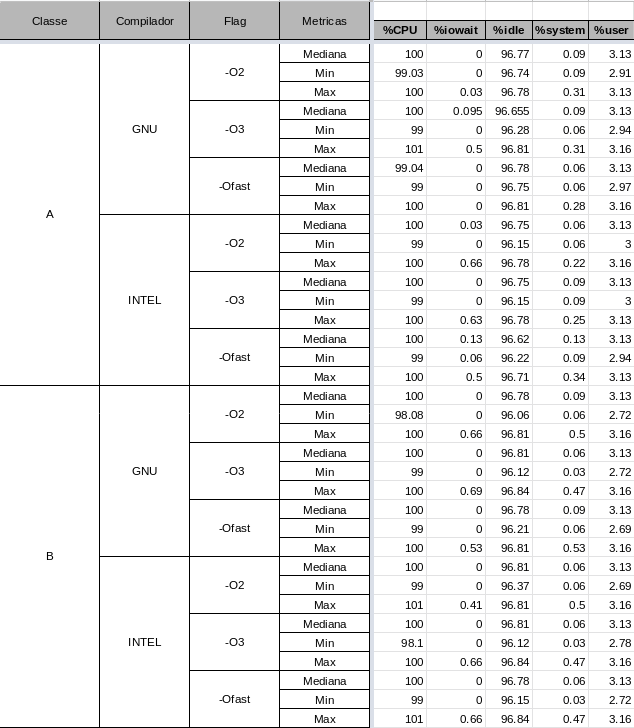
\includegraphics[width=12cm]{Pictures/FT_r641_SER_CPU.png}
    \caption{Implementação SER: Utilização CPU}
    \label{figure:FT_r641_SER_CPU}
\end{figure}

\begin{figure}[H]
    \centering
    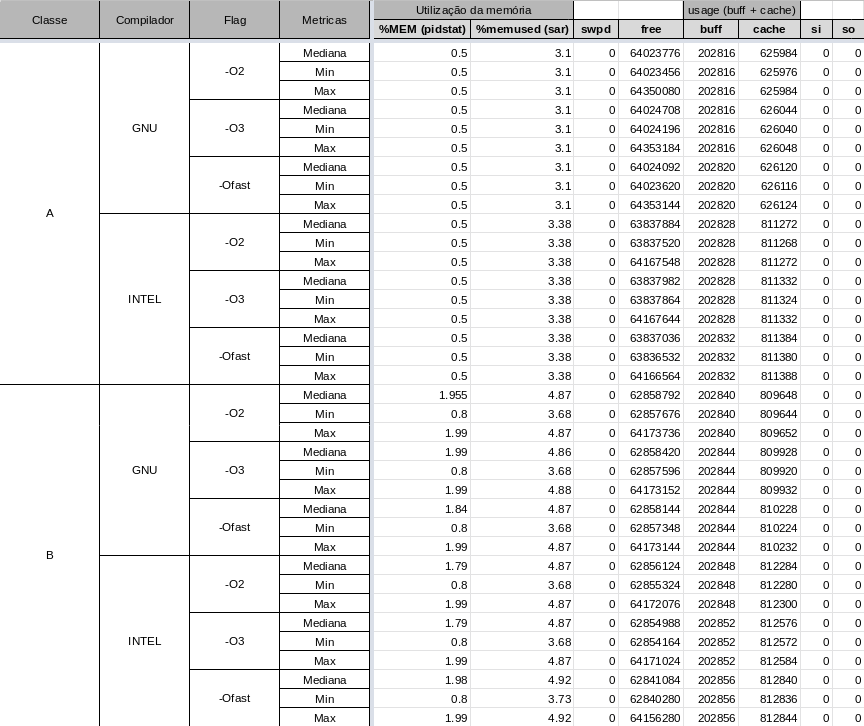
\includegraphics[width=12cm]{Pictures/FT_r641_SER_MEM.png}
    \caption{Implementação SER: Utilização Memória}
    \label{figure:FT_r641_SER_MEM}
\end{figure}

\begin{figure}[H]
    \centering
    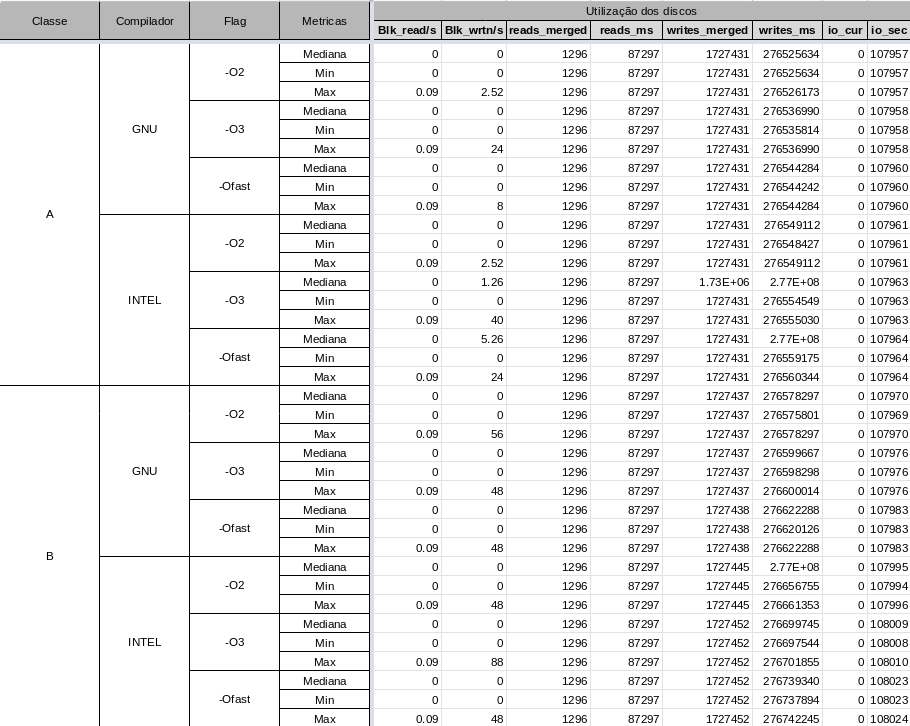
\includegraphics[width=12cm]{Pictures/FT_r641_SER_DISK.png}
    \caption{Implementação SER: Utilização Disco}
    \label{figure:FT_r641_SER_DISK}
\end{figure}

\begin{figure}[H]
    \centering
    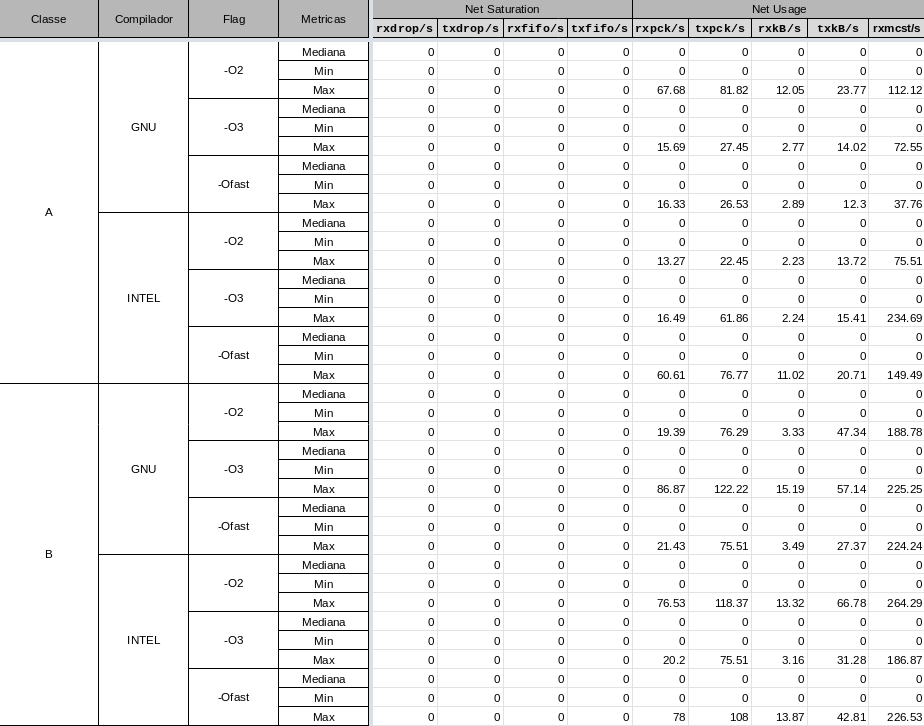
\includegraphics[width=12cm]{Pictures/FT_r641_SER_NET.png}
    \caption{Implementação SER: Saturação/Utilização Rede}
    \label{figure:FT_r641_SER_NT}
\end{figure}



\begin{figure}[H]
    \centering
    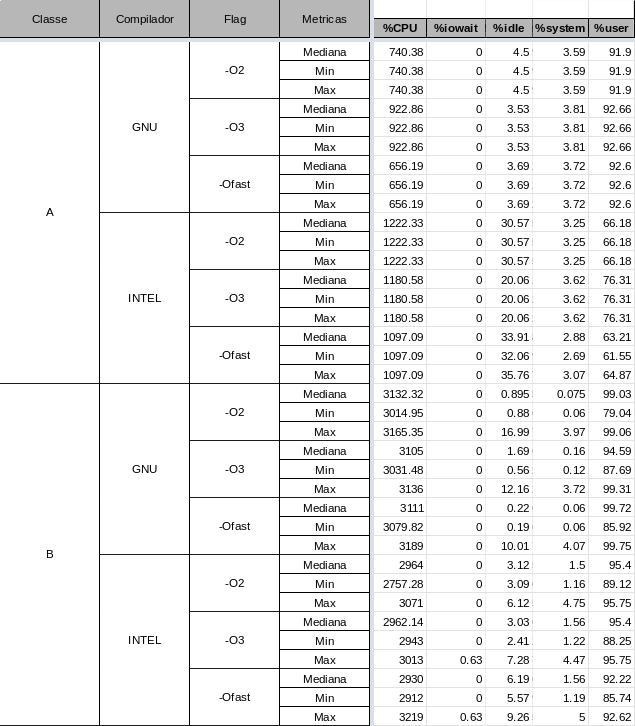
\includegraphics[width=12cm]{Pictures/FT_r641_OMP_CPU.png}
    \caption{Implementação OMP: Utilização CPU}
    \label{figure:FT_r641_OMP_CPU}
\end{figure}

\begin{figure}[H]
    \centering
    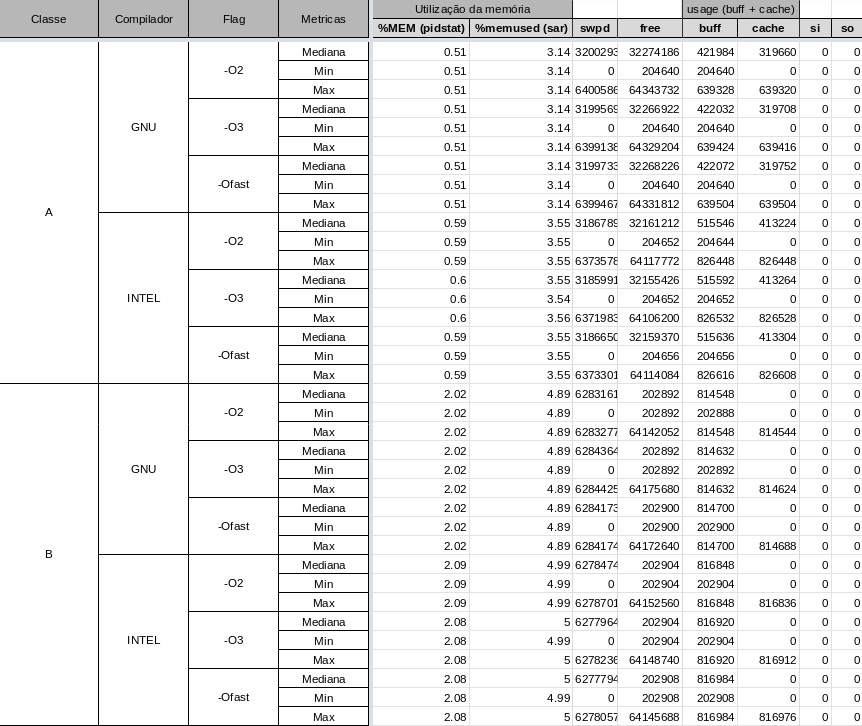
\includegraphics[width=12cm]{Pictures/FT_r641_OMP_MEM.png}
    \caption{Implementação OMP: Utilização Memória}
    \label{figure:FT_r641_OMP_MEM}
\end{figure}

\begin{figure}[H]
    \centering
    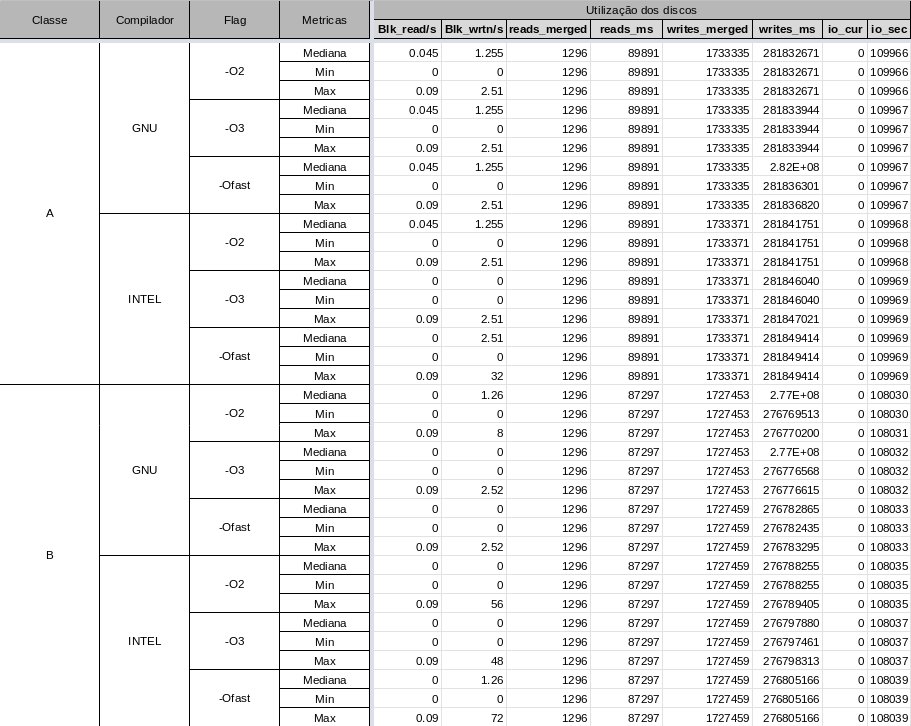
\includegraphics[width=12cm]{Pictures/FT_r641_OMP_DISK.png}
    \caption{Implementação OMP: Utilização Disco}
    \label{figure:FT_r641_OMP_DISK}
\end{figure}

\begin{figure}[H]
    \centering
    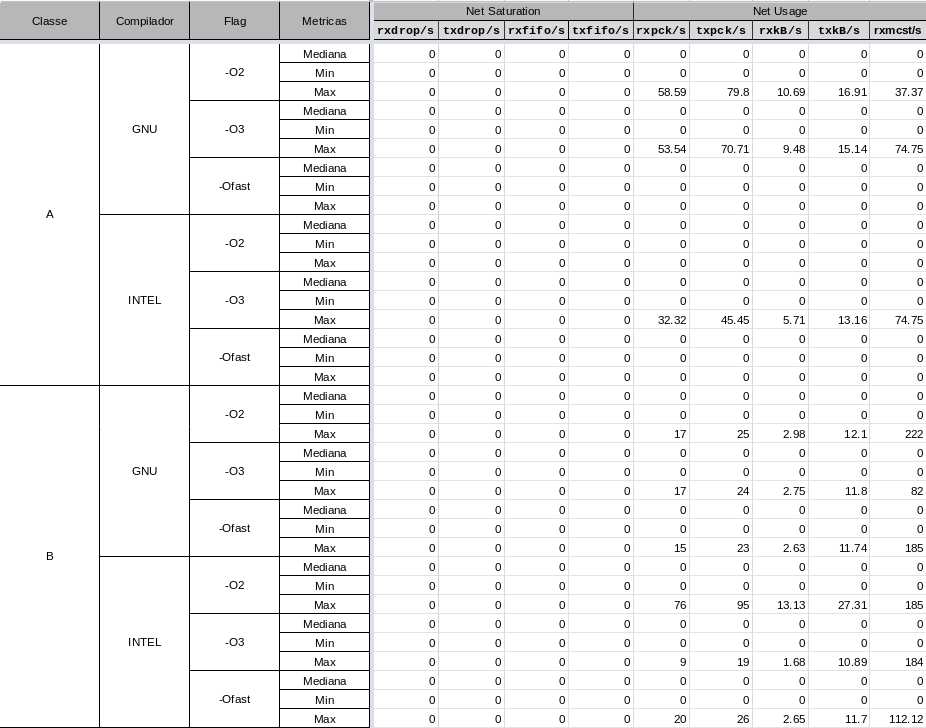
\includegraphics[width=12cm]{Pictures/FT_r641_OMP_NET.png}
    \caption{Implementação OMP: Saturação/Utilização Rede}
    \label{figure:FT_r641_OMP_NET}
\end{figure}



\begin{figure}[H]
    \centering
    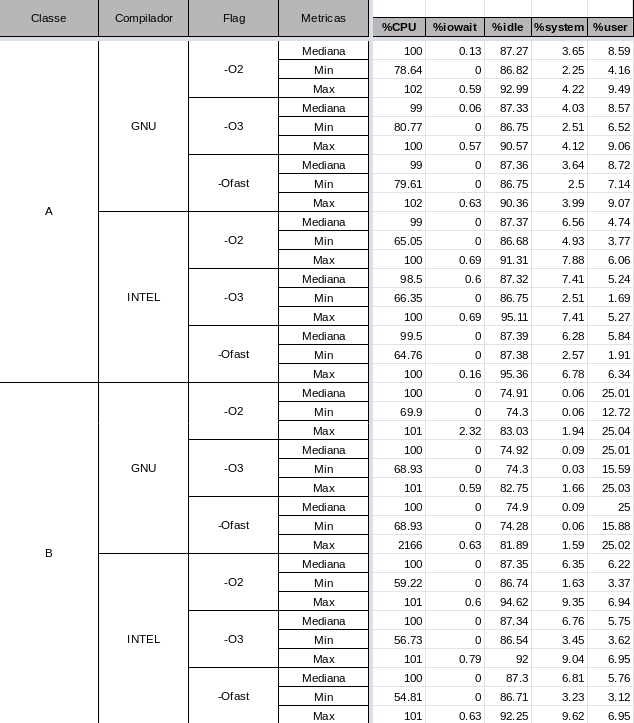
\includegraphics[width=12cm]{Pictures/FT_r641_MPIE_CPU.png}
    \caption{Implementação MPI Ethernet: Utilização CPU}
    \label{figure:FT_r641_MPIE_CPU}
\end{figure}

\begin{figure}[H]
    \centering
    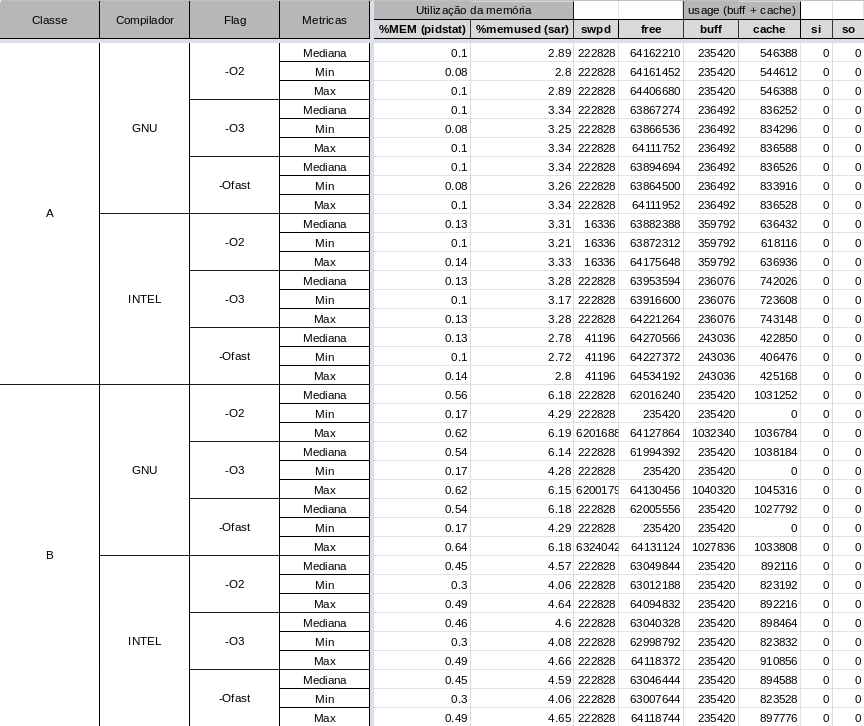
\includegraphics[width=12cm]{Pictures/FT_r641_MPIE_MEM.png}
    \caption{Implementação MPI Ethernet: Utilização Memória}
    \label{figure:FT_r641_MPIE_MEM}
\end{figure}

\begin{figure}[H]
    \centering
    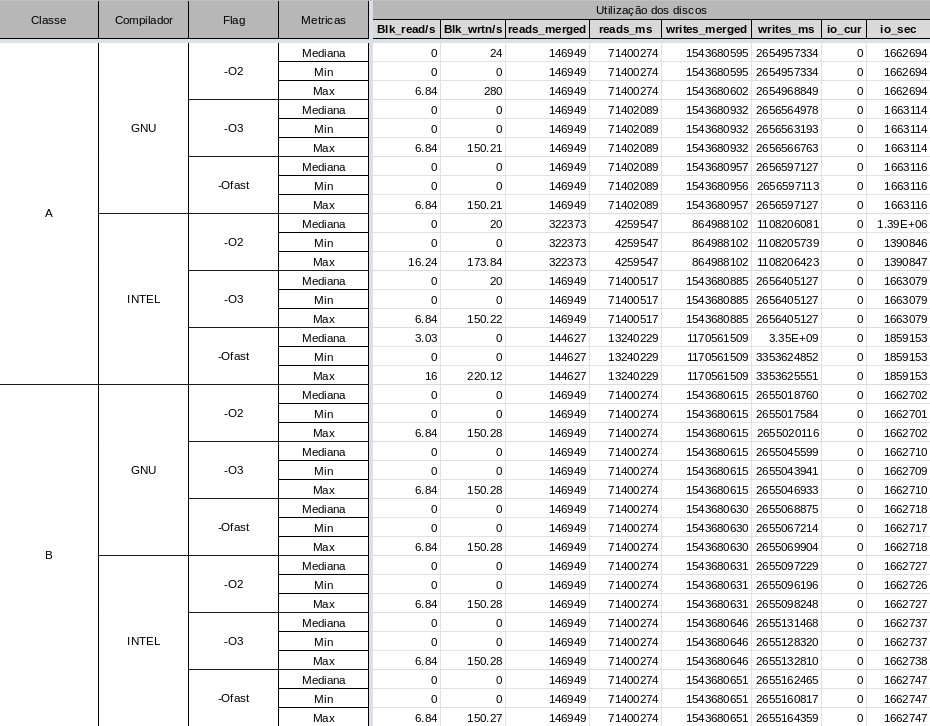
\includegraphics[width=12cm]{Pictures/FT_r641_MPIE_DISK.png}
    \caption{Implementação MPI Ethernet: Utilização Disco}
    \label{figure:FT_r641_MPIE_DISK}
\end{figure}

\begin{figure}[H]
    \centering
    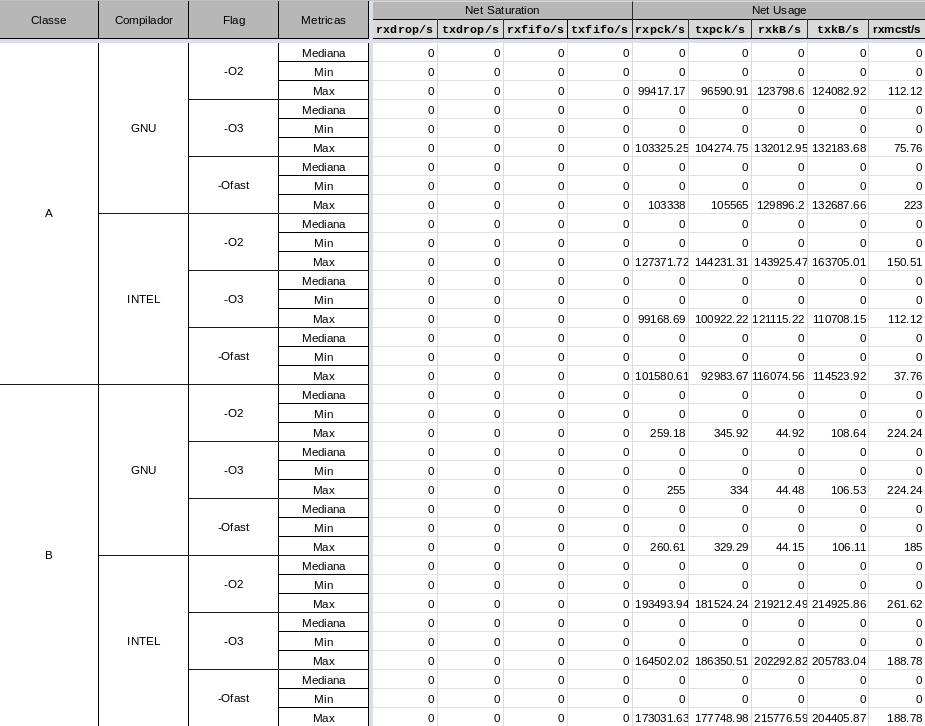
\includegraphics[width=12cm]{Pictures/FT_r641_MPIE_NET.png}
    \caption{Implementação MPI Ethernet: Saturação/Utilização Rede}
    \label{figure:FT_r641_MPIE_NET}
\end{figure}

\subsubsection{Nodo r431}

\begin{figure}[H]
    \centering
    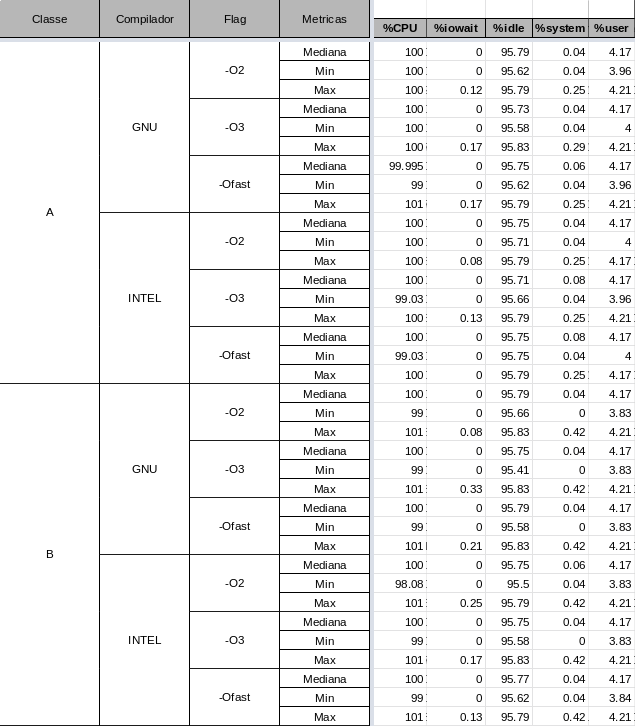
\includegraphics[width=12cm]{Pictures/FT_r431_SER_CPU.png}
    \caption{Implementação SER: Utilização CPU}
    \label{figure:FT_r431_SER_CPU}
\end{figure}

\begin{figure}[H]
    \centering
    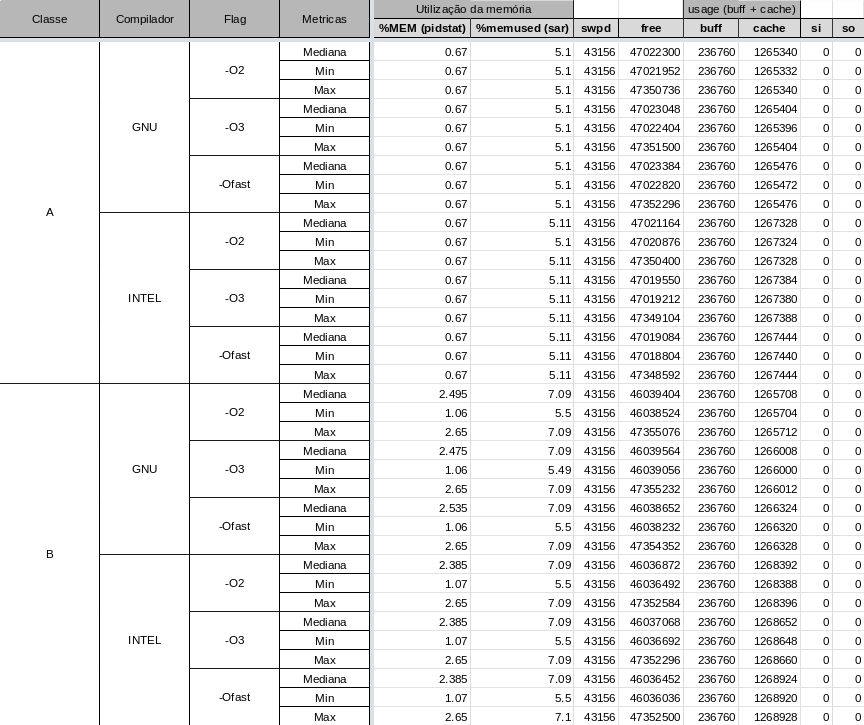
\includegraphics[width=12cm]{Pictures/FT_r431_SER_MEM.png}
    \caption{Implementação SER: Utilização Memória}
    \label{figure:FT_r431_SER_MEM}
\end{figure}

\begin{figure}[H]
    \centering
    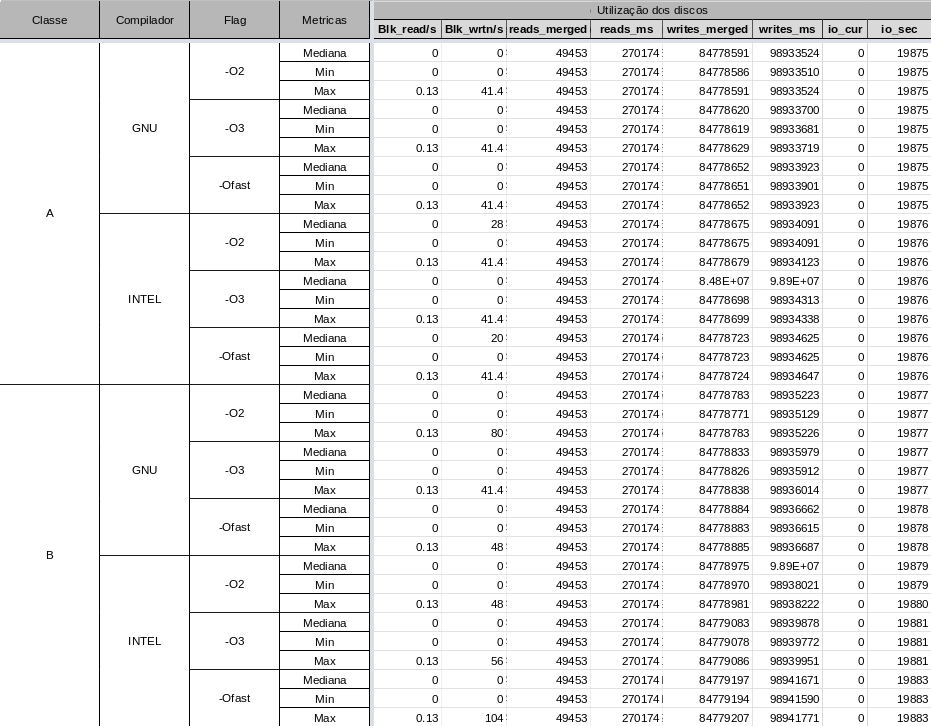
\includegraphics[width=12cm]{Pictures/FT_r431_SER_DISK.png}
    \caption{Implementação SER: Utilização Disco}
    \label{figure:FT_r431_SER_DISK}
\end{figure}

\begin{figure}[H]
    \centering
    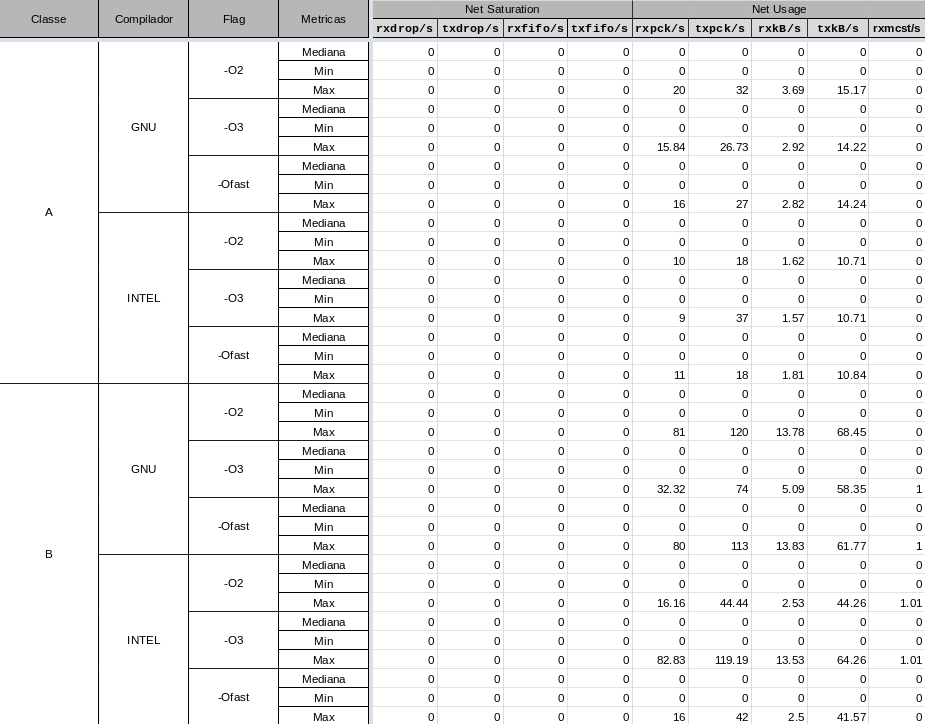
\includegraphics[width=12cm]{Pictures/FT_r431_SER_NET.png}
    \caption{Implementação SER: Saturação/Utilização Rede}
    \label{figure:FT_r431_SER_NT}
\end{figure}



\begin{figure}[H]
    \centering
    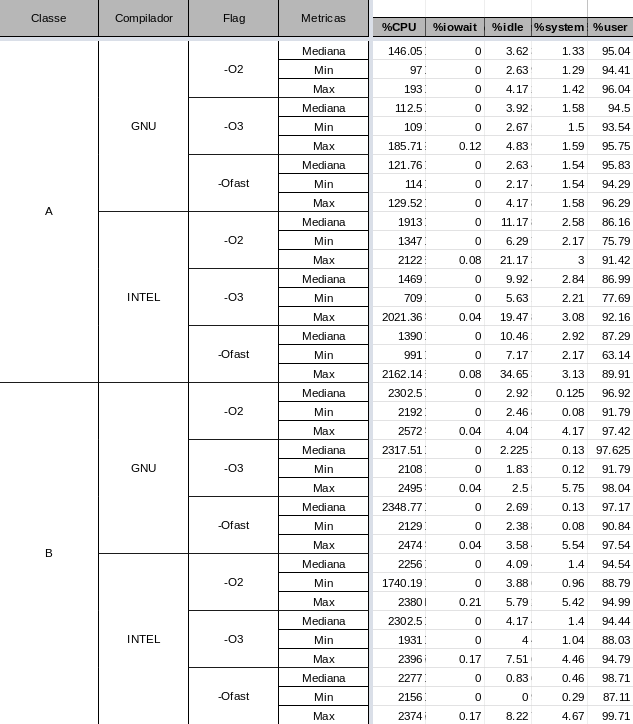
\includegraphics[width=12cm]{Pictures/FT_r431_OMP_CPU.png}
    \caption{Implementação OMP: Utilização CPU}
    \label{figure:FT_r431_OMP_CPU}
\end{figure}

\begin{figure}[H]
    \centering
    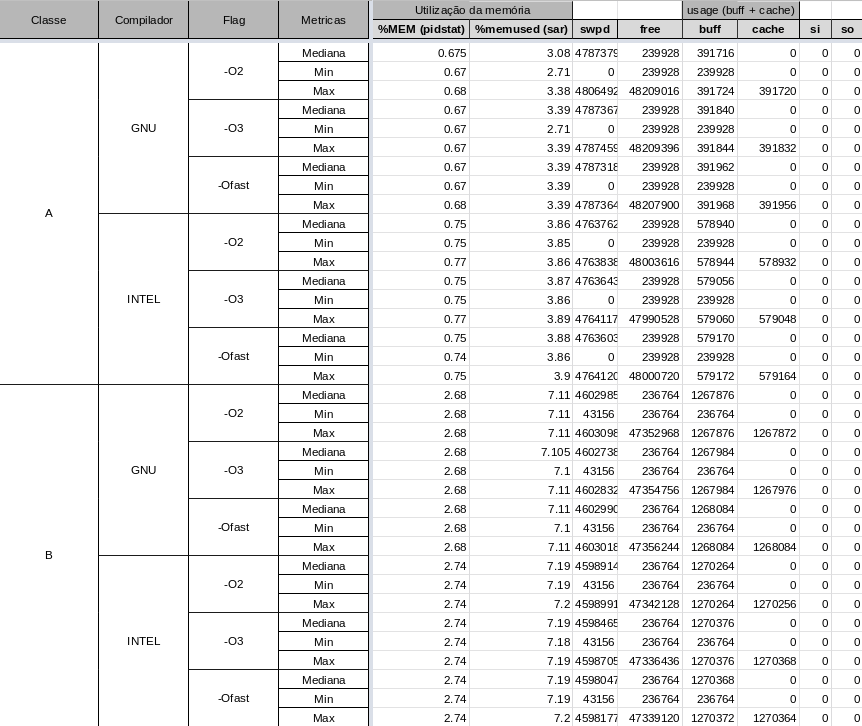
\includegraphics[width=12cm]{Pictures/FT_r431_OMP_MEM.png}
    \caption{Implementação OMP: Utilização Memória}
    \label{figure:FT_r431_OMP_MEM}
\end{figure}

\begin{figure}[H]
    \centering
    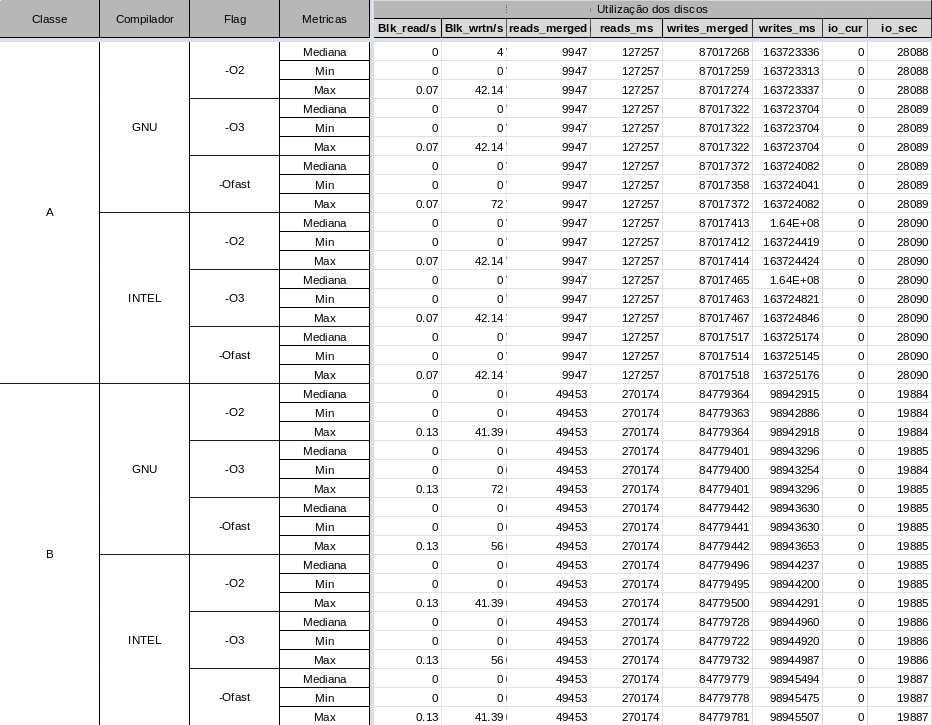
\includegraphics[width=12cm]{Pictures/FT_r431_OMP_DISK.png}
    \caption{Implementação OMP: Utilização Disco}
    \label{figure:FT_r431_OMP_DISK}
\end{figure}

\begin{figure}[H]
    \centering
    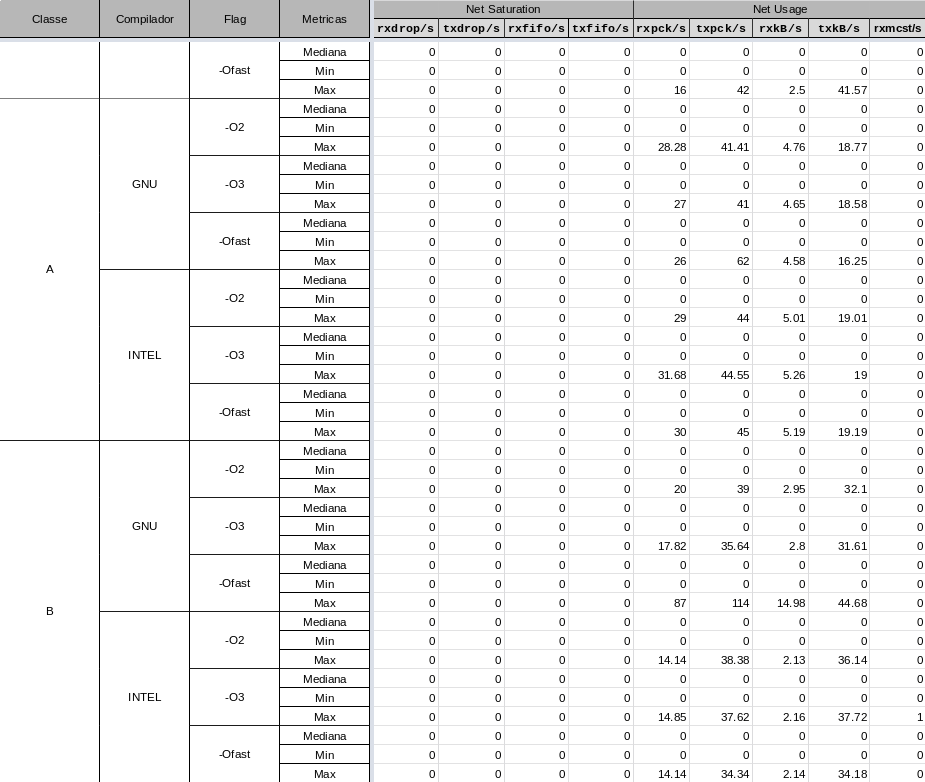
\includegraphics[width=12cm]{Pictures/FT_r431_OMP_NET.png}
    \caption{Implementação OMP: Saturação/Utilização Rede}
    \label{figure:FT_r431_OMP_NET}
\end{figure}



\begin{figure}[H]
    \centering
    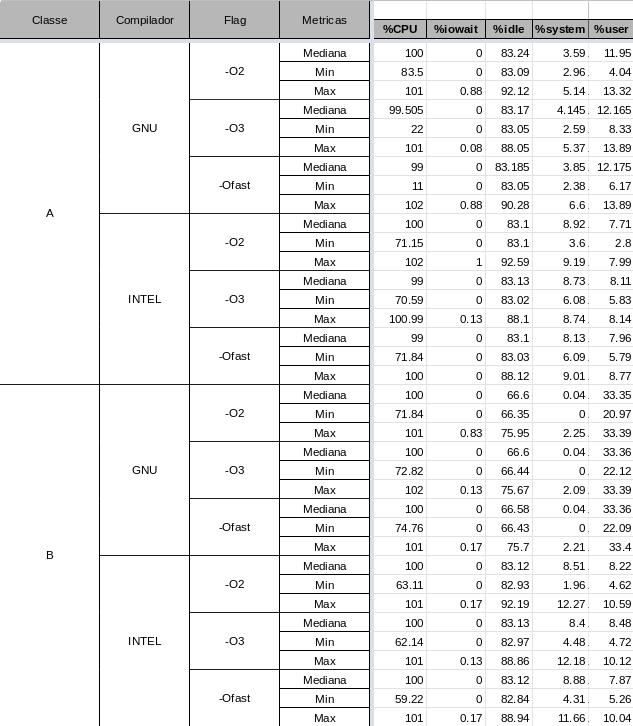
\includegraphics[width=12cm]{Pictures/FT_r431_MPIE_CPU.png}
    \caption{Implementação MPI Ethernet: Utilização CPU}
    \label{figure:FT_r431_MPIE_CPU}
\end{figure}

\begin{figure}[H]
    \centering
    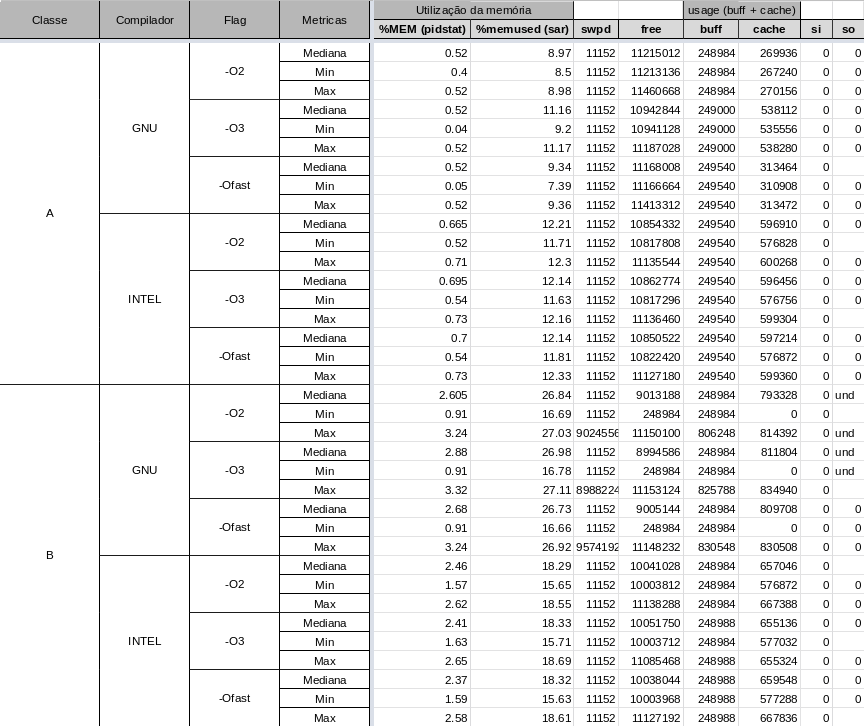
\includegraphics[width=12cm]{Pictures/FT_r431_MPIE_MEM.png}
    \caption{Implementação MPI Ethernet: Utilização Memória}
    \label{figure:FT_r431_MPIE_MEM}
\end{figure}

\begin{figure}[H]
    \centering
    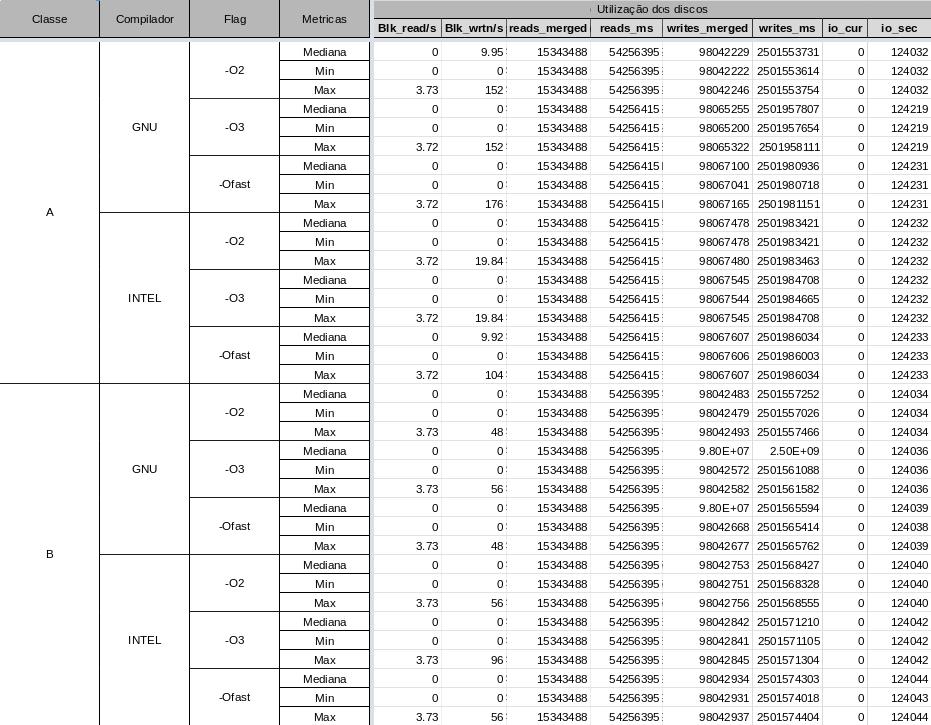
\includegraphics[width=12cm]{Pictures/FT_r431_MPIE_DISK.png}
    \caption{Implementação MPI Ethernet: Utilização Disco}
    \label{figure:FT_r431_MPIE_DISK}
\end{figure}

\begin{figure}[H]
    \centering
    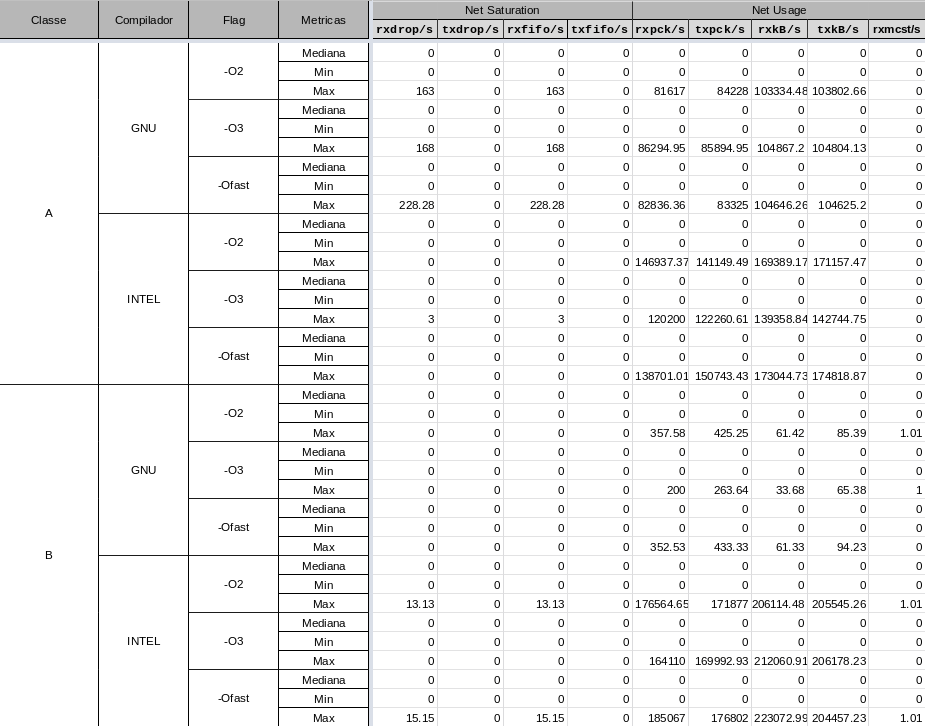
\includegraphics[width=12cm]{Pictures/FT_r431_MPIE_NET.png} 
    \caption{Implementação MPI Ethernet: Saturação/Utilização Rede}
    \label{figure:FT_r431_MPIE_NET}
\end{figure}

\subsection{Benchmark LU-MZ}

\subsubsection{Nodo r641}

\begin{figure}[H]
    \centering
    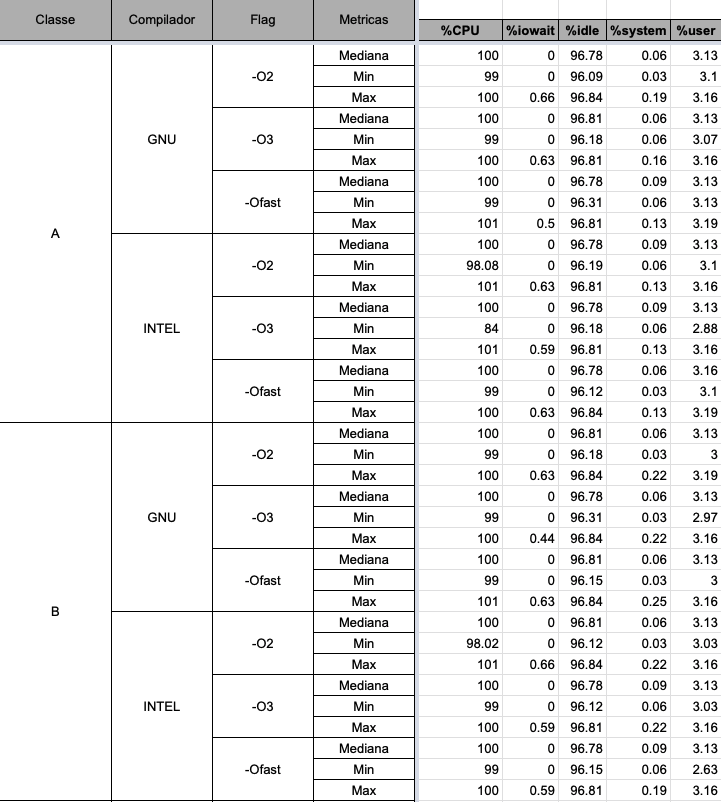
\includegraphics[width=12cm]{Pictures/LUMZ_r641_SER_CPU.png}
    \caption{Implementação SER: Utilização CPU}
    \label{figure:LUMZ_r641_SER_CPU}
\end{figure}

\begin{figure}[H]
    \centering
    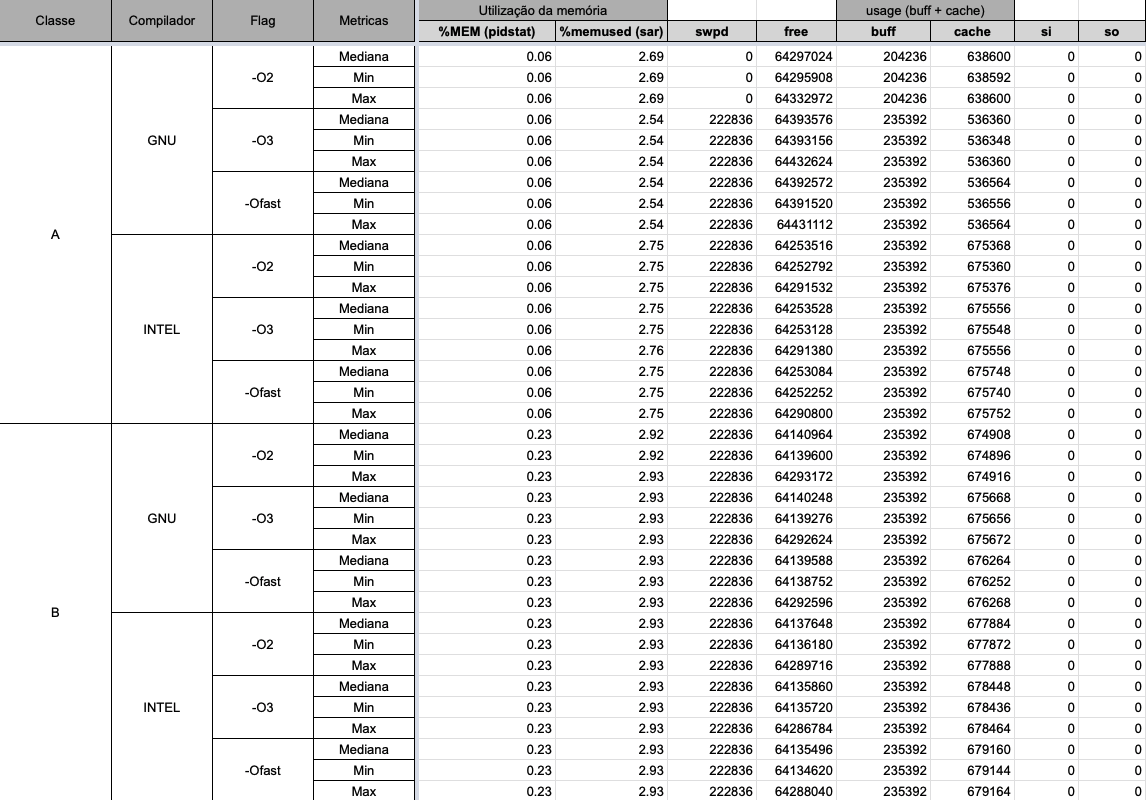
\includegraphics[width=12cm]{Pictures/LUMZ_r641_SER_MEM.png}
    \caption{Implementação SER: Utilização Memória}
    \label{figure:LUMZ_r641_SER_MEM}
\end{figure}

\begin{figure}[H]
    \centering
    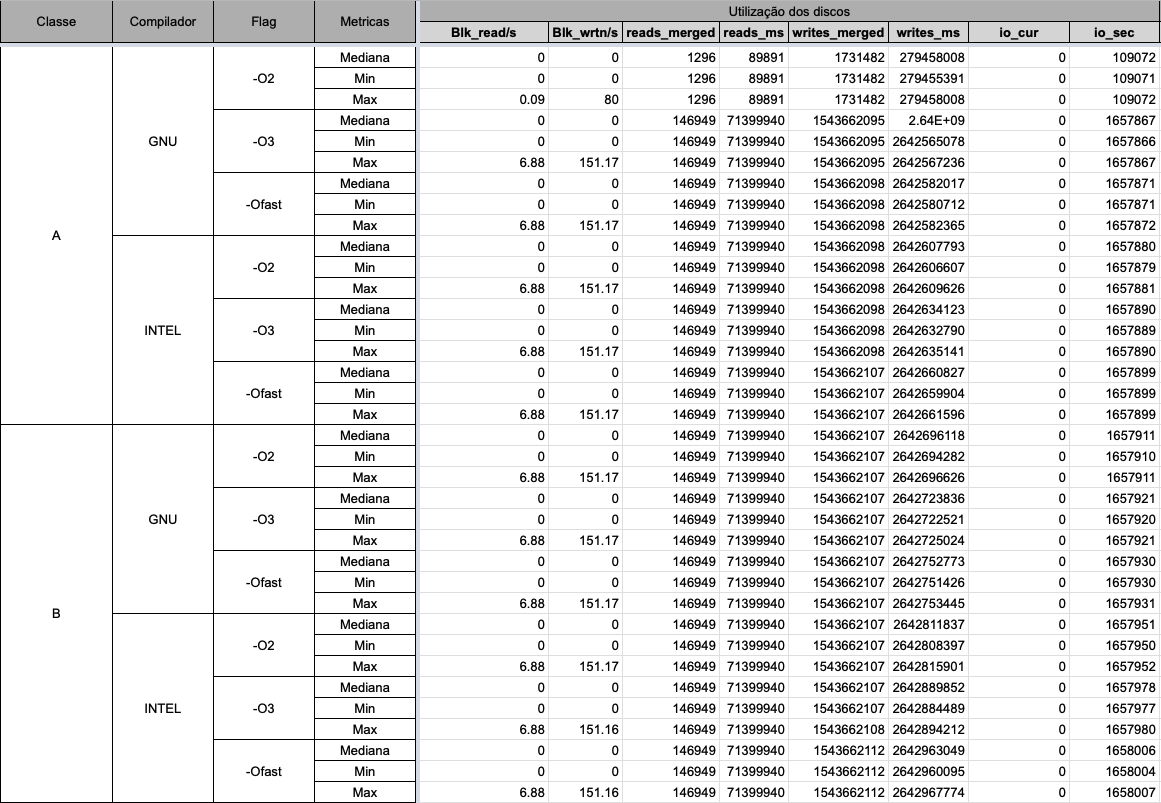
\includegraphics[width=12cm]{Pictures/LUMZ_r641_SER_DISK.png}
    \caption{Implementação SER: Utilização Disco}
    \label{figure:LUMZ_r641_SER_DISK}
\end{figure}

\begin{figure}[H]
    \centering
    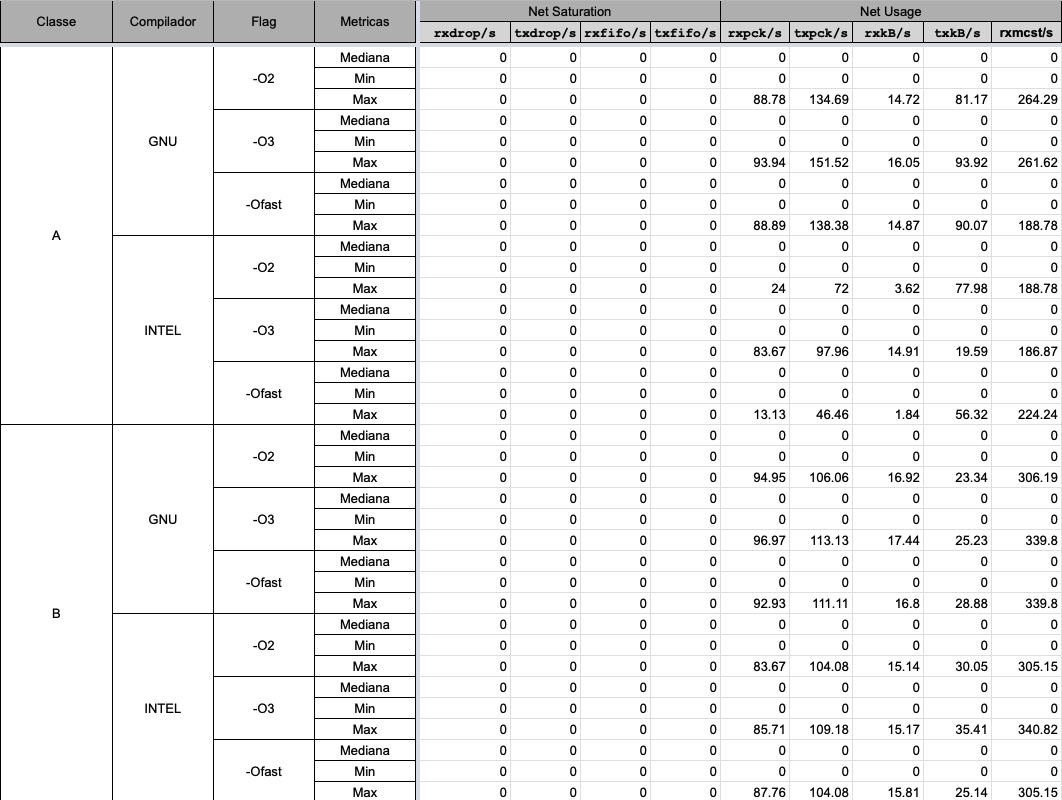
\includegraphics[width=12cm]{Pictures/LUMZ_r641_SER_NET.png}
    \caption{Implementação SER: Saturação/Utilização Rede}
    \label{figure:LUMZ_r641_SER_NT}
\end{figure}



\begin{figure}[H]
    \centering
    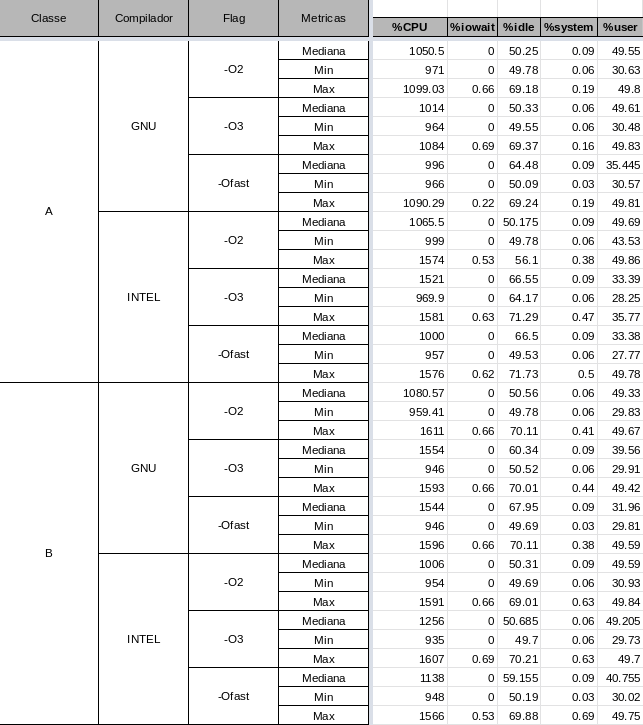
\includegraphics[width=12cm]{Pictures/LUMZ_r641_OMP_CPU.png}
    \caption{Implementação OMP: Utilização CPU}
    \label{figure:LUMZ_r641_OMP_CPU}
\end{figure}

\begin{figure}[H]
    \centering
    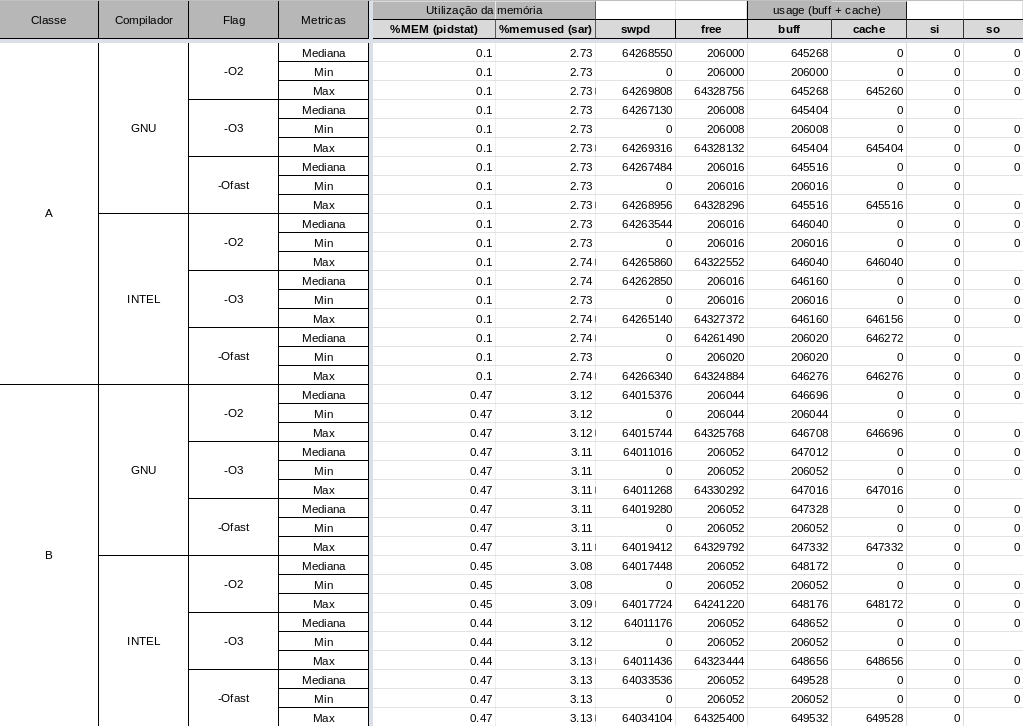
\includegraphics[width=12cm]{Pictures/LUMZ_r641_OMP_MEM.png}
    \caption{Implementação OMP: Utilização Memória}
    \label{figure:LUMZ_r641_OMP_MEM}
\end{figure}

\begin{figure}[H]
    \centering
    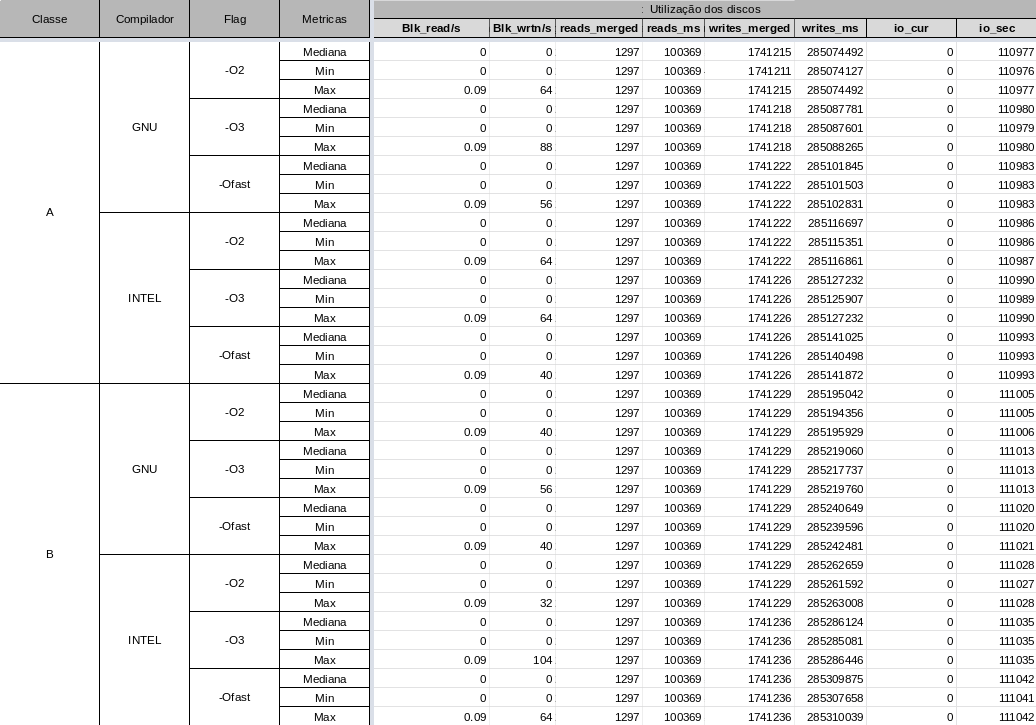
\includegraphics[width=12cm]{Pictures/LUMZ_r641_OMP_DISK.png}
    \caption{Implementação OMP: Utilização Disco}
    \label{figure:LUMZ_r641_OMP_DISK}
\end{figure}

\begin{figure}[H]
    \centering
    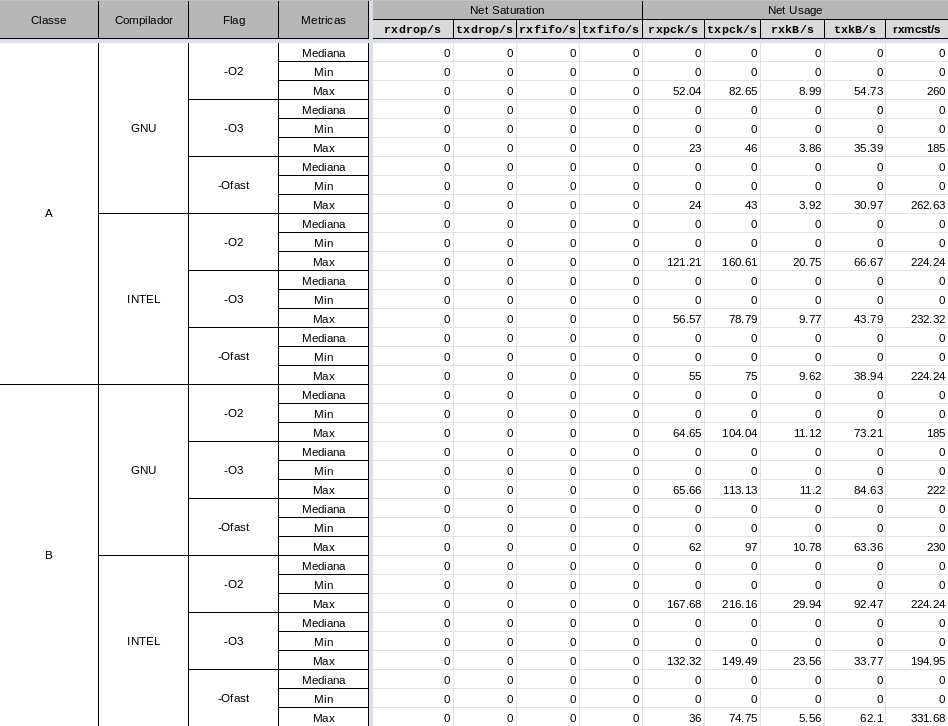
\includegraphics[width=12cm]{Pictures/LUMZ_r641_OMP_NET.png}
    \caption{Implementação OMP: Saturação/Utilização Rede}
    \label{figure:LUMZ_r641_OMP_NET}
\end{figure}



\begin{figure}[H]
    \centering
    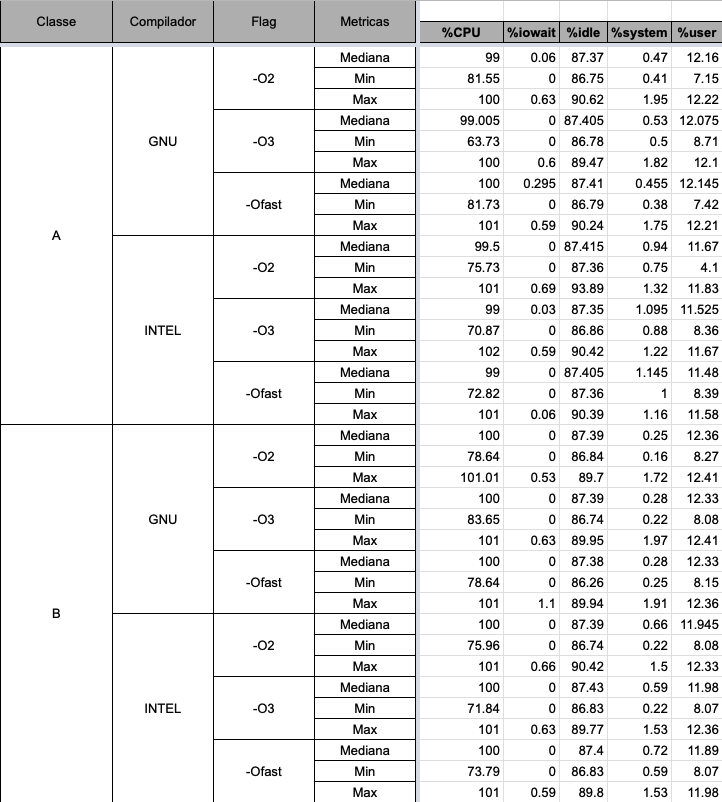
\includegraphics[width=12cm]{Pictures/LUMZ_r641_MPIE_CPU.png}
    \caption{Implementação MPI Ethernet: Utilização CPU}
    \label{figure:LUMZ_r641_MPIE_CPU}
\end{figure}

\begin{figure}[H]
    \centering
    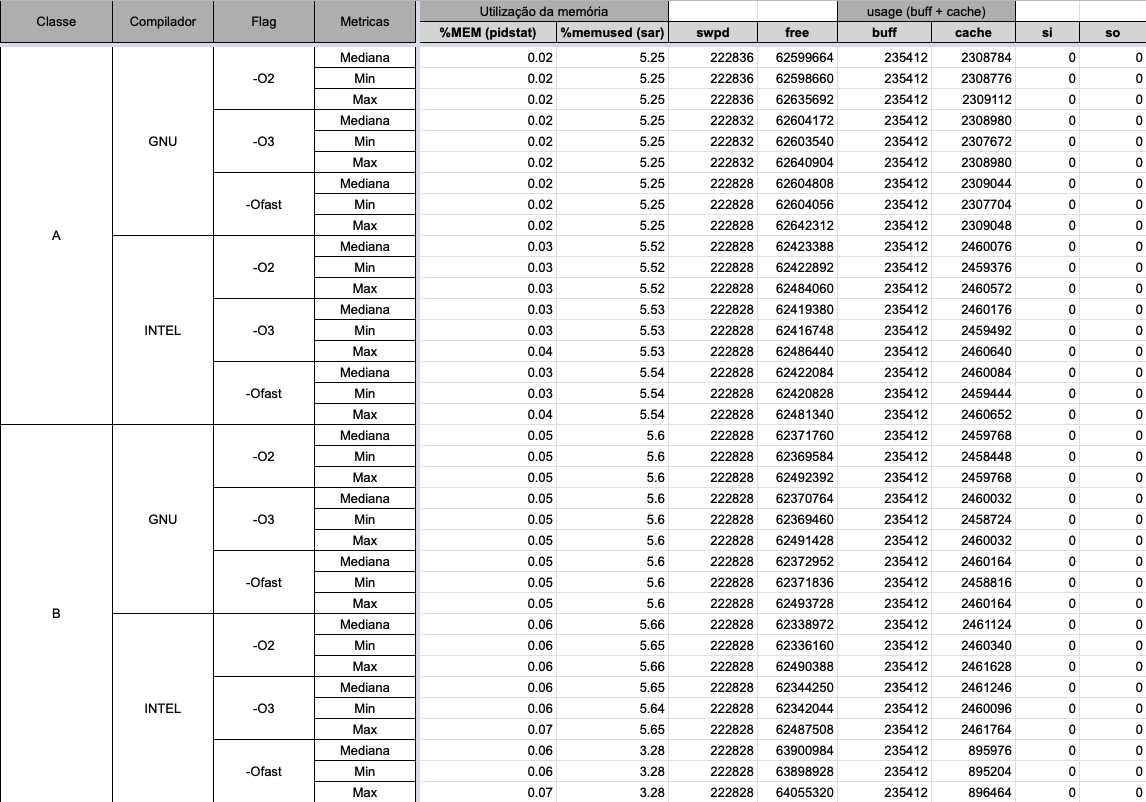
\includegraphics[width=12cm]{Pictures/LUMZ_r641_MPIE_MEM.png}
    \caption{Implementação MPI Ethernet: Utilização Memória}
    \label{figure:LUMZ_r641_MPIE_MEM}
\end{figure}

\begin{figure}[H]
    \centering
    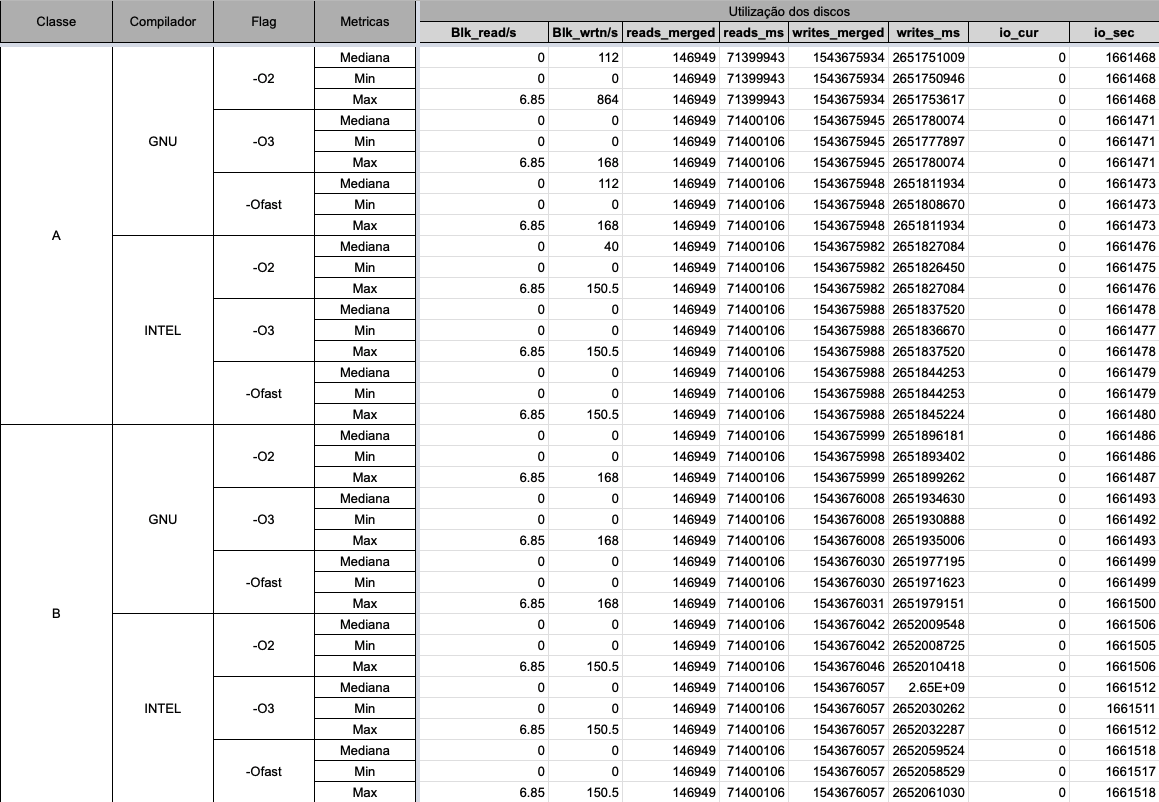
\includegraphics[width=12cm]{Pictures/LUMZ_r641_MPIE_DISK.png}
    \caption{Implementação MPI Ethernet: Utilização Disco}
    \label{figure:LUMZ_r641_MPIE_DISK}
\end{figure}

\begin{figure}[H]
    \centering
    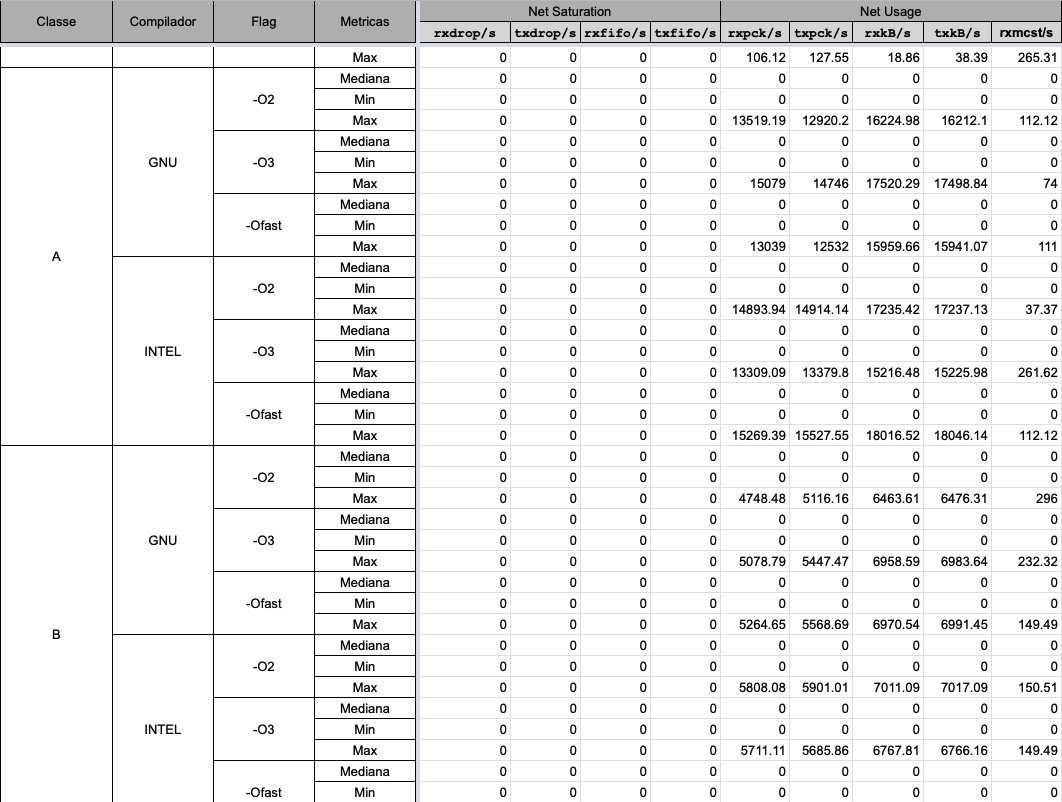
\includegraphics[width=12cm]{Pictures/LUMZ_r641_MPIE_NET.png}
    \caption{Implementação MPI Ethernet: Saturação/Utilização Rede}
    \label{figure:LUMZ_r641_MPIE_NET}
\end{figure}

\subsubsection{Nodo r431}

\begin{figure}[H]
    \centering
    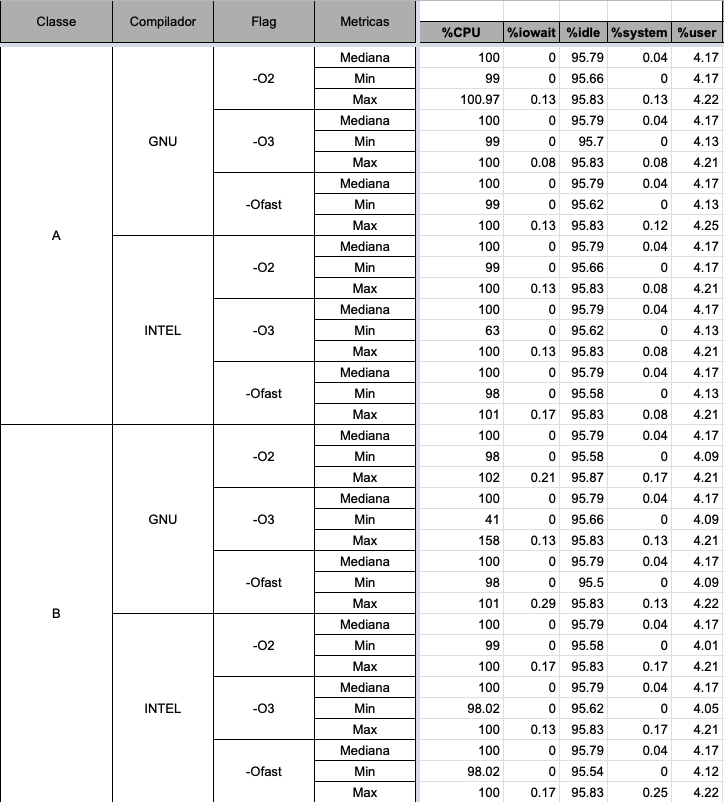
\includegraphics[width=12cm]{Pictures/LUMZ_r431_SER_CPU.png}
    \caption{Implementação SER: Utilização CPU}
    \label{figure:LUMZ_r431_SER_CPU}
\end{figure}

\begin{figure}[H]
    \centering
    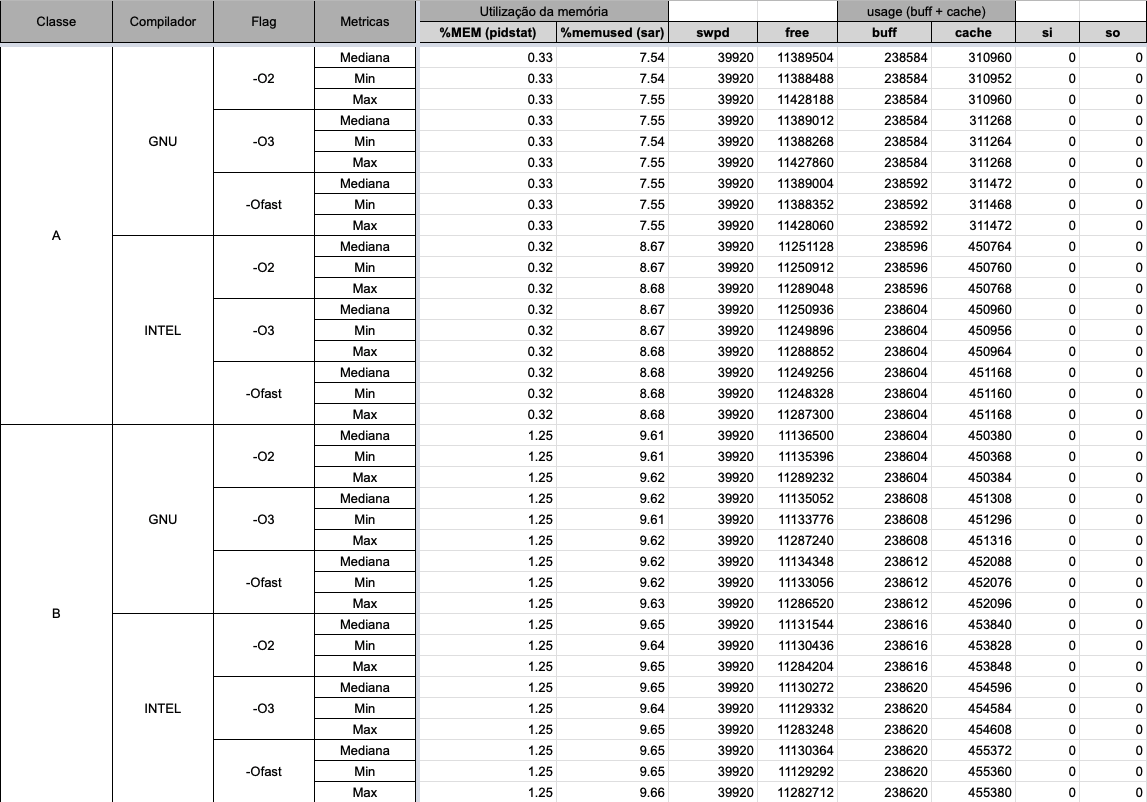
\includegraphics[width=12cm]{Pictures/LUMZ_r431_SER_MEM.png}
    \caption{Implementação SER: Utilização Memória}
    \label{figure:LUMZ_r431_SER_MEM}
\end{figure}

\begin{figure}[H]
    \centering
    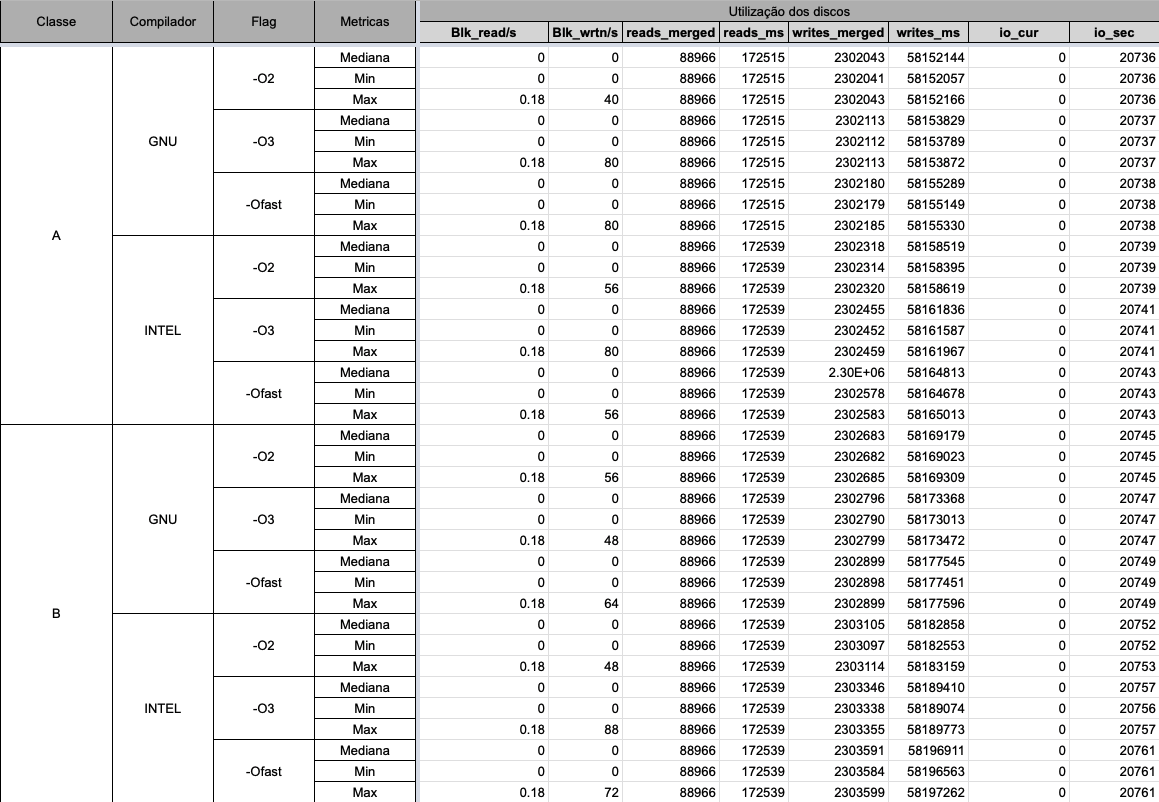
\includegraphics[width=12cm]{Pictures/LUMZ_r431_SER_DISK.png}
    \caption{Implementação SER: Utilização Disco}
    \label{figure:LUMZ_r431_SER_DISK}
\end{figure}

\begin{figure}[H]
    \centering
    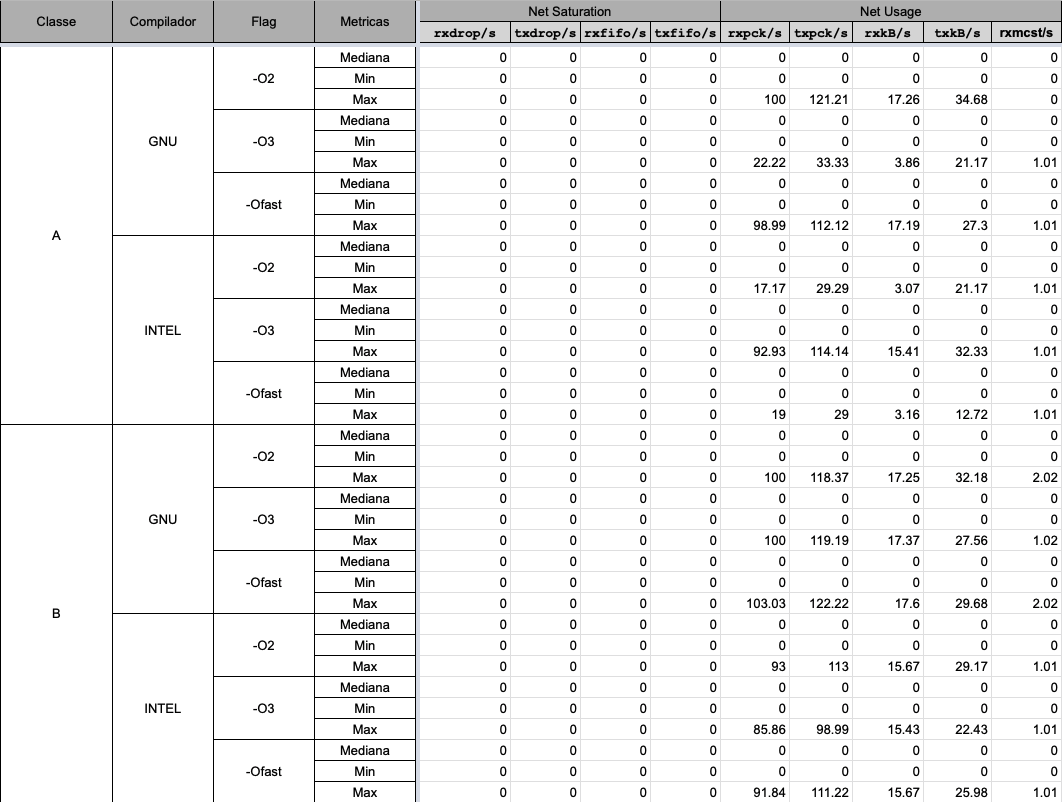
\includegraphics[width=12cm]{Pictures/LUMZ_r431_SER_NET.png}
    \caption{Implementação SER: Saturação/Utilização Rede}
    \label{figure:LUMZ_r431_SER_NT}
\end{figure}

\begin{figure}[H]
    \centering
    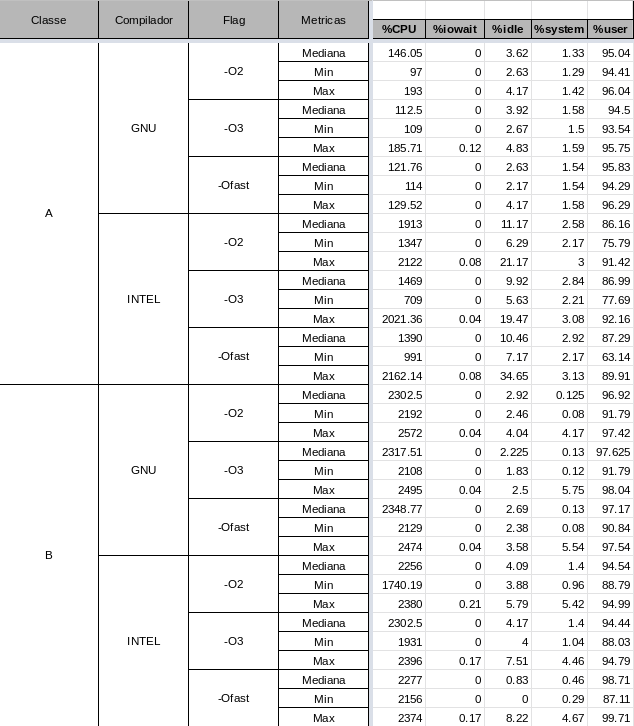
\includegraphics[width=12cm]{Pictures/LUMZ_r431_OMP_CPU.png}
    \caption{Implementação OMP: Utilização CPU}
    \label{figure:LUMZ_r431_OMP_CPU}
\end{figure}

\begin{figure}[H]
    \centering
    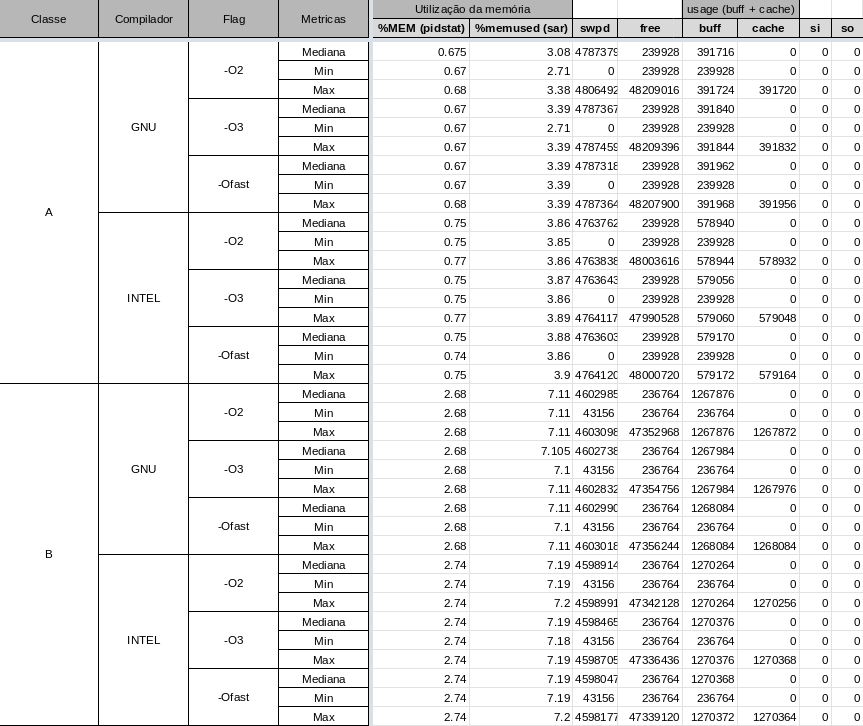
\includegraphics[width=12cm]{Pictures/LUMZ_r431_OMP_MEM.png}
    \caption{Implementação OMP: Utilização Memória}
    \label{figure:LUMZ_r431_OMP_MEM}
\end{figure}

\begin{figure}[H]
    \centering
    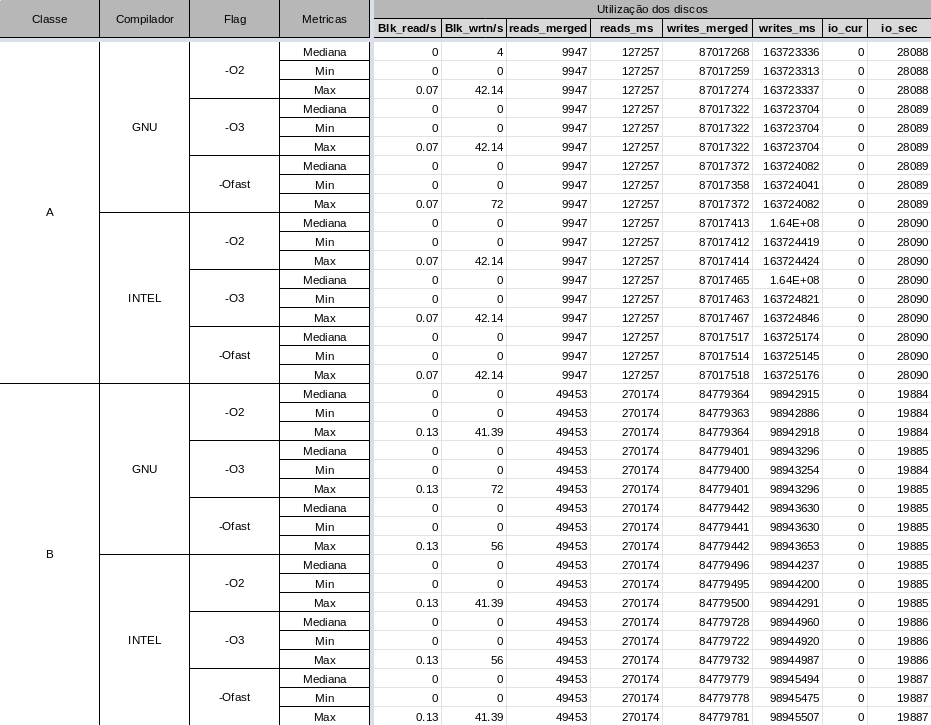
\includegraphics[width=12cm]{Pictures/LUMZ_r431_OMP_DISK.png}
    \caption{Implementação OMP: Utilização Disco}
    \label{figure:LUMZ_r431_OMP_DISK}
\end{figure}

\begin{figure}[H]
    \centering
    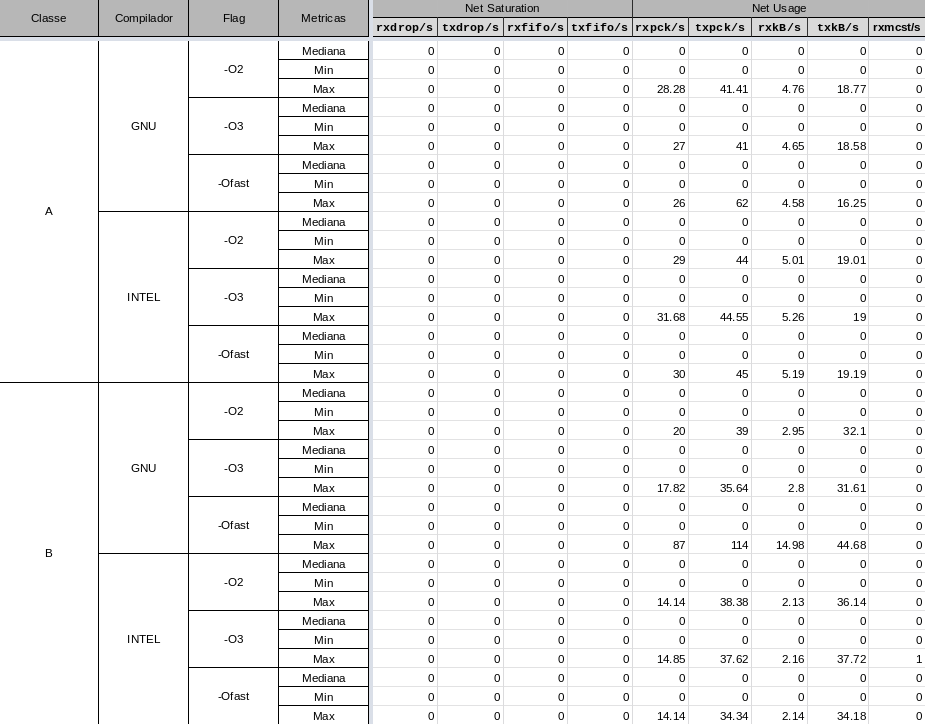
\includegraphics[width=12cm]{Pictures/LUMZ_r431_OMP_NET.png}
    \caption{Implementação OMP: Saturação/Utilização Rede}
    \label{figure:LUMZ_r431_OMP_NET}
\end{figure}

\begin{figure}[H]
    \centering
    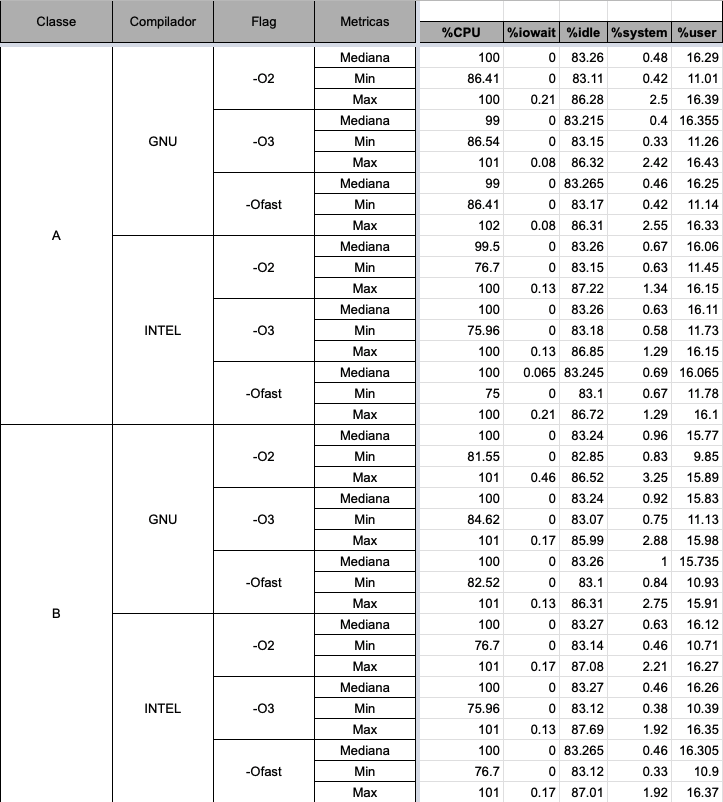
\includegraphics[width=12cm]{Pictures/LUMZ_r431_MPIE_CPU.png}
    \caption{Implementação MPI Ethernet: Utilização CPU}
    \label{figure:LUMZ_r431_MPIE_CPU}
\end{figure}

\begin{figure}[H]
    \centering
    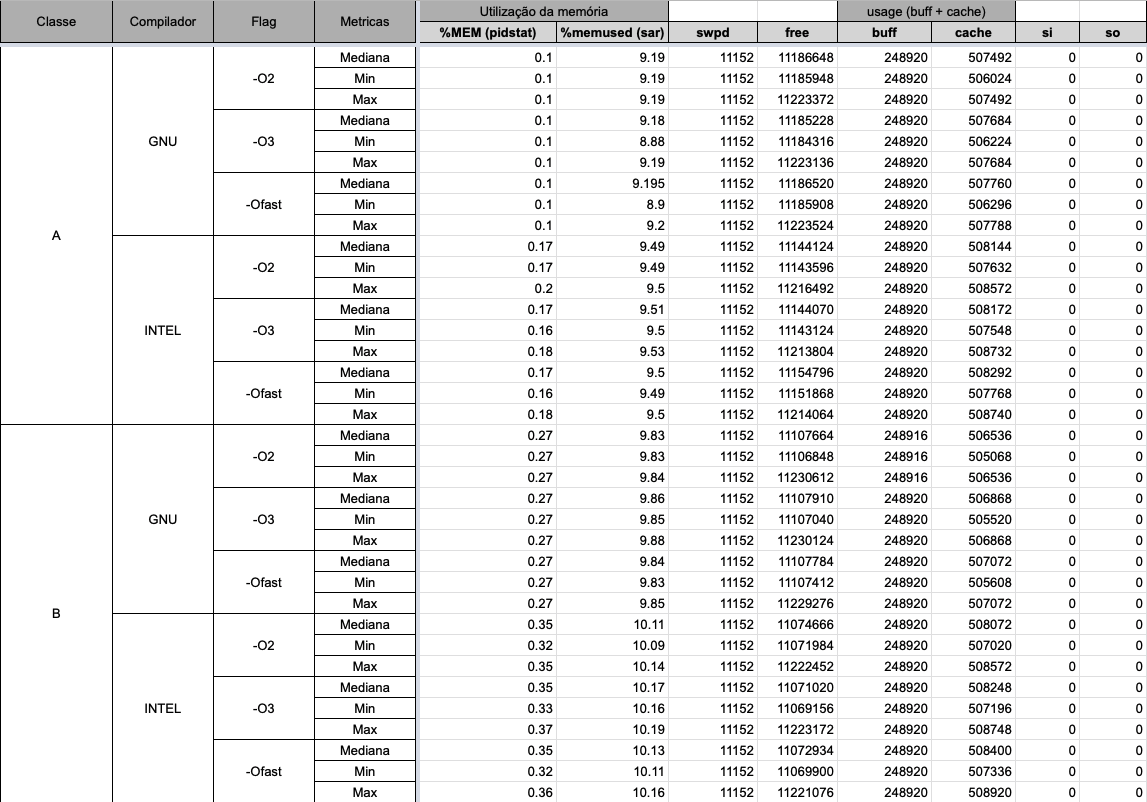
\includegraphics[width=12cm]{Pictures/LUMZ_r431_MPIE_MEM.png}
    \caption{Implementação MPI Ethernet: Utilização Memória}
    \label{figure:LUMZ_r431_MPIE_MEM}
\end{figure}

\begin{figure}[H]
    \centering
    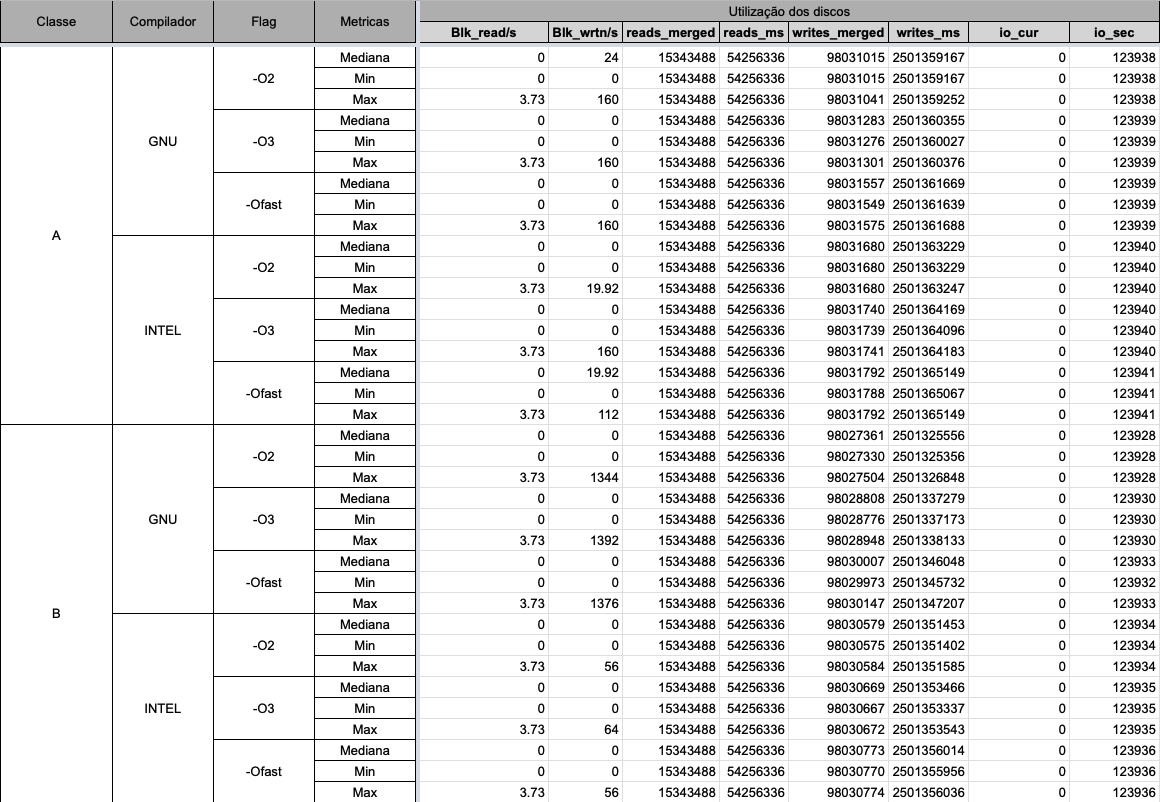
\includegraphics[width=12cm]{Pictures/LUMZ_r431_MPIE_DISK.png}
    \caption{Implementação MPI Ethernet: Utilização Disco}
    \label{figure:LUMZ_r431_MPIE_DISK}
\end{figure}

\begin{figure}[H]
    \centering
    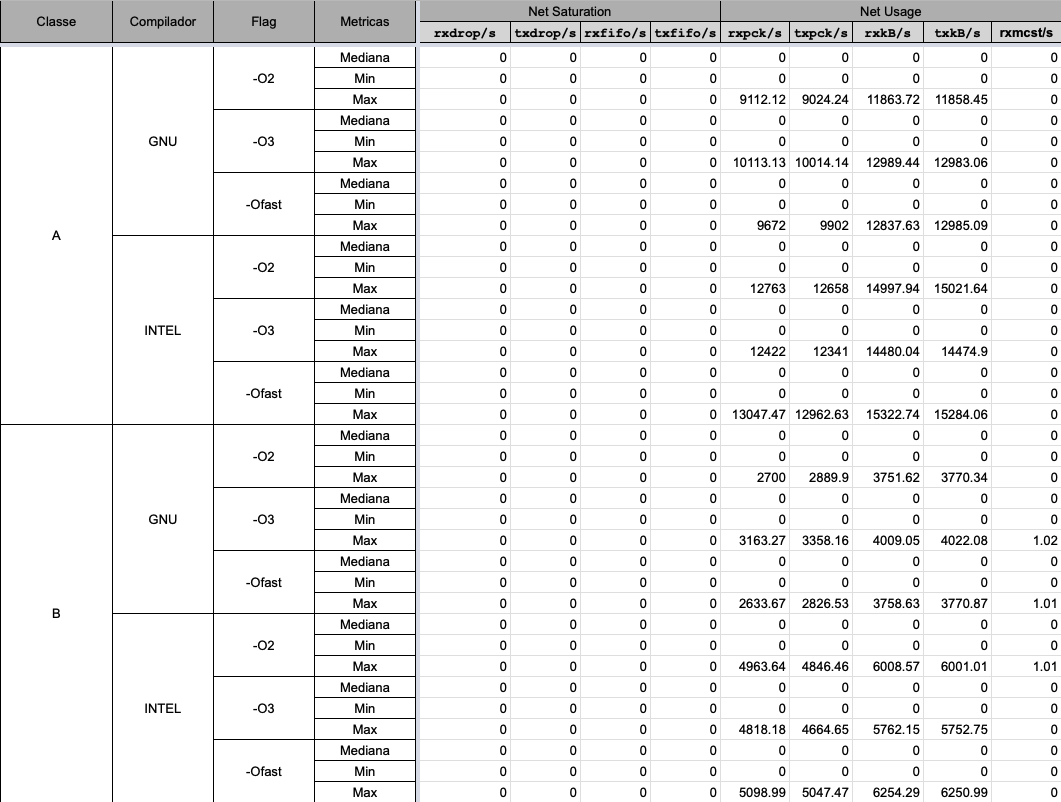
\includegraphics[width=12cm]{Pictures/LUMZ_r431_MPIE_NET.png}
    \caption{Implementação MPI Ethernet: Saturação/Utilização Rede}
    \label{figure:LUMZ_r431_MPIE_NET}
\end{figure}

\section{Comparação de resultados}
\subsection{Implementações: SER vs. OMP vs. MPI}

\subsubsection{FT}

\begin{figure}[H]
    \centering
    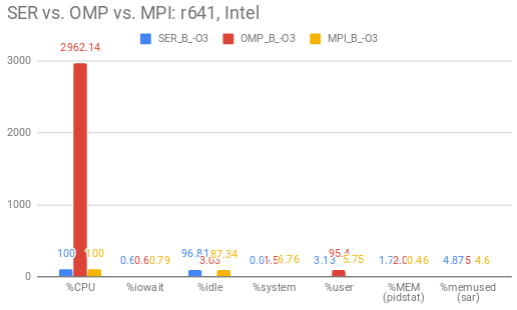
\includegraphics[width=12cm]{Pictures/FT_SER_OMP_MPI_r641_Intel_Comp.png}
    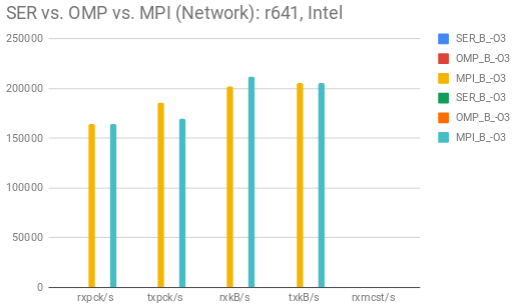
\includegraphics[width=12cm]{Pictures/FT_SER_OMP_MPI_r641_Intel_Comm.png}
    \caption{r641: Compilador Intel}
    \label{fig:ft_ser_omp_mpi_r641_intel}
\end{figure}

\begin{figure}[H]
    \centering
    \includegraphics[width=12cm]{Pictures/FT_SER_OMP_MPI_r641_GNU_Comp.png}
    \includegraphics[width=12cm]{Pictures/FT_SER_OMP_MPI_r641_GNU_Comm.png}
    \caption{r641: Compilador GNU}
    \label{fig:ft_ser_omp_mpi_r641_gnu}
\end{figure}

\begin{figure}[H]
    \centering
    \includegraphics[width=12cm]{Pictures/FT_SER_OMP_MPI_r431_Intel_Comp.png}
    \includegraphics[width=12cm]{Pictures/FT_SER_OMP_MPI_r431_Intel_Comm.png}
    \caption{r431: Compilador Intel}
    \label{fig:ft_ser_omp_mpi_r431_intel}
\end{figure}

\begin{figure}[H]
    \centering
    \includegraphics[width=12cm]{Pictures/FT_SER_OMP_MPI_r431_GNU_Comp.png}
    \includegraphics[width=12cm]{Pictures/FT_SER_OMP_MPI_r431_GNU_Comm.png}
    \caption{r431: Compilador GNU}
    \label{fig:ft_ser_omp_mpi_r431_gnu}
\end{figure}

\subsubsection{LUMZ}

\begin{figure}[H]
    \centering
    \includegraphics[width=12cm]{Pictures/LUMZ_SER_OMP_MPI_r641_Intel_Comp.png}
    \includegraphics[width=12cm]{Pictures/LUMZ_SER_OMP_MPI_r641_Intel_Comm.png}
    \caption{r641: Compilador Intel}
    \label{fig:lumz_ser_omp_mpi_r641_intel}
\end{figure}

\begin{figure}[H]
    \centering
    \includegraphics[width=12cm]{Pictures/LUMZ_SER_OMP_MPI_r641_GNU_Comp.png}
    \includegraphics[width=12cm]{Pictures/LUMZ_SER_OMP_MPI_r641_GNU_Comm.png}
    \caption{r641: Compilador GNU}
    \label{fig:lumz_ser_omp_mpi_r641_gnu}
\end{figure}

\begin{figure}[H]
    \centering
    \includegraphics[width=12cm]{Pictures/LUMZ_SER_OMP_MPI_r431_Intel_Comp.png}
    \includegraphics[width=12cm]{Pictures/LUMZ_SER_OMP_MPI_r431_Intel_Comm.png}
    \caption{r431: Compilador Intel}
    \label{fig:lumz_ser_omp_mpi_r431_intel}
\end{figure}

\begin{figure}[H]
    \centering
    \includegraphics[width=12cm]{Pictures/LUMZ_SER_OMP_MPI_r431_GNU_Comp.png}
    \includegraphics[width=12cm]{Pictures/LUMZ_SER_OMP_MPI_r431_GNU_Comm.png}
    \caption{r431: Compilador GNU}
    \label{fig:lumz_ser_omp_mpi_r431_gnu}
\end{figure}

\subsection{Classes: A vs. B}
\subsubsection{FT}

\begin{figure}[H]
    \centering
    \includegraphics[width=12cm]{Pictures/FT_A_B_r641_Intel.png}
    \caption{r641: Compilador Intel}
    \label{fig:ft_A_B_r641_intel}
\end{figure}

\begin{figure}[H]
    \centering
    \includegraphics[width=12cm]{Pictures/FT_A_B_r641_GNU.png}
    \caption{r641: Compilador GNU}
    \label{fig:ft_A_B_r641_gnu}
\end{figure}

\begin{figure}[H]
    \centering
    \includegraphics[width=12cm]{Pictures/FT_A_B_r431_Intel.png}
    \caption{r431: Compilador Intel}
    \label{fig:ft_A_B_r431_intel}
\end{figure}

\begin{figure}[H]
    \centering
    \includegraphics[width=12cm]{Pictures/FT_A_B_r431_GNU.png}
    \caption{r431: Compilador GNU}
    \label{fig:ft_A_B_r431_gnu}
\end{figure}

\subsubsection{LUMZ}
\begin{figure}[H]
    \centering
    \includegraphics[width=12cm]{Pictures/LUMZ_A_B_r641_Intel.png}
    \caption{r641: Compilador Intel}
    \label{fig:lumz_A_B_r641_intel}
\end{figure}

\begin{figure}[H]
    \centering
    \includegraphics[width=12cm]{Pictures/LUMZ_A_B_r641_GNU.png}
    \caption{r641: Compilador GNU}
    \label{fig:lumz_A_B_r641_gnu}
\end{figure}

\begin{figure}[H]
    \centering
    \includegraphics[width=12cm]{Pictures/LUMZ_A_B_r431_Intel.png}
    \caption{r431: Compilador Intel}
    \label{fig:lumz_A_B_r431_intel}
\end{figure}

\begin{figure}[H]
    \centering
    \includegraphics[width=12cm]{Pictures/LUMZ_A_B_r431_GNU.png}
    \caption{r431: Compilador GNU}
    \label{fig:lumz_A_B_r431_gnu}
\end{figure}


\subsection{Compiladores: GNU vs. Intel}
\subsubsection{FT}

\begin{figure}[H]
    \centering
    \includegraphics[width=13cm]{Pictures/FT_GNU_Intel_r641.png}
    \caption{r641: Classe B}
    \label{fig:ft_gnu_intel_r641}
\end{figure}

\begin{figure}[H]
    \centering
    \includegraphics[width=13cm]{Pictures/FT_GNU_Intel_r431.png}
    \caption{r431: Classe B}
    \label{fig:ft_gnu_intel_r431}
\end{figure}

\subsubsection{LUMZ}

\begin{figure}[H]
    \centering
    \includegraphics[width=13cm]{Pictures/LUMZ_GNU_Intel_r641.png}
    \caption{r641: Classe B}
    \label{fig:lumz_gnu_intel_r641}
\end{figure}

\begin{figure}[H]
    \centering
    \includegraphics[width=13cm]{Pictures/LUMZ_GNU_Intel_r431.png}
    \caption{r431: Classe B}
    \label{fig:lumz_gnu_intel_r431}
\end{figure}

\subsection{Nodos: r641 vs. r431}

\subsubsection{FT}

\begin{figure}[H]
    \centering
    \includegraphics[width=12cm]{Pictures/FT_r641_r431_Comp.png}
    \includegraphics[width=12cm]{Pictures/FT_r641_r431_Comm.png}
    \caption{r641 vs. r431}
    \label{fig:FT_r641_r431}
\end{figure}

\subsubsection{LUMZ}
\begin{figure}[H]
    \centering
    \includegraphics[width=12cm]{Pictures/LUMZ_r641_r431_Comp.png}
    \includegraphics[width=12cm]{Pictures/LUMZ_r641_r431_Comm.png}
    \caption{r641 vs. r431}
    \label{fig:LUMZ_r641_r431}
\end{figure}


\subsection{Benchmarks: FT vs. LUMZ}
\begin{figure}[H]
    \centering
    \includegraphics[width=12cm]{Pictures/FT_LUMZ_r641_Intel_Comp.png}
    \includegraphics[width=12cm]{Pictures/FT_LUMZ_r641_Intel_Comm.png}
    \caption{FT vs. LUMZ; r641; Intel}
    \label{fig:FT_LUMZ_r641}
\end{figure}

\begin{figure}[H]
    \centering
    \includegraphics[width=12cm]{Pictures/FT_LUMZ_r431_Intel_Comp.png}
    \includegraphics[width=12cm]{Pictures/FT_LUMZ_r431_Intel_Comm.png}
    \caption{FT vs. LUMZ; r431; Intel}
    \label{fig:FT_LUMZ_r431}
\end{figure}

\section{Scripts}

\subsection{Script para FT}\label{FTscript}
\begin{minted}{bash}
#!/bin/bash

function getB(){
    CUR_RESULT_DIR=$RESULT_DIR/$6/$5/$1_$2_$3_$4_results
    mkdir -p $CUR_RESULT_DIR

    CMDS=("sar -r 1 -u"
    "vmstat 1"
    "pidstat -u 1"
    "pidstat -r 1"
    "sar -r 1"
    "iostat -d 1"
    "vmstat -d 1"
    "sar -r 1 -n DEV"
    "sar -r 1 -n EDEV")

    OUTPUT_DIR=("$CUR_RESULT_DIR/cpu_sar.txt"
    "$CUR_RESULT_DIR/mem_vmstat.txt"
    "$CUR_RESULT_DIR/cpu_pidstat.txt"
    "$CUR_RESULT_DIR/mem_pidstat.txt"
    "$CUR_RESULT_DIR/mem_sar.txt"
    "$CUR_RESULT_DIR/disk_iostat.txt"
    "$CUR_RESULT_DIR/disk_vmstat.txt"
    "$CUR_RESULT_DIR/network_usage_sar.txt"
    "$CUR_RESULT_DIR/network_saturation_sar.txt")

    for (( i = 0; i < ${#CMDS[@]}; i++ ))
    do
        ${CMDS[$i]} > ${OUTPUT_DIR[$i]} &
        PID=($!)
        if [[ $5 == "NPB3.3-MPI" ]]; then
            if [[ $1 == "INTEL" ]]; then
                if [[ $6 == "FTr641Myri" ]]; then
                    module load intel/openmpi_mx/1.8.2
                    source /share/apps/intel/parallel_studio_xe_2019/compilers_and_libraries
_2019/linux/bin/compilervars.sh intel64
                    mpirun -rr -genv I_MPI_FABRICS mx -np 8 ./ft.$4.8
                else
                    module load intel/openmpi_eth/1.8.2
                    source /share/apps/intel/parallel_studio_xe_2019/compilers_and_libraries
_2019/linux/bin/compilervars.sh intel64
                    mpirun -rr -np 8 ./ft.$4.8
                fi
            else
                if [[ $6 == "FTr641Myri" ]]; then
                    module load gnu/openmpi_mx/1.8.2
                    module load gcc/5.3.0
                    mpirun --map-by node --mca mtl mx --mca pml cm -np 8 ./ft.$4.8
                else
                    module load gnu/openmpi_eth/1.8.2
                    module load gcc/5.3.0
                    mpirun --map-by node -np 8 ./ft.$4.8
                fi
            fi
        else
            ./ft.$4.x
        fi
        kill -9 $PID
    done

}


function bench(){
    mkdir bin
    
    if [[ $1 == "INTEL" ]]; then
        if [[ $5 == "NPB3.3-MPI" ]]; then
            if [[ $6 == "FTr641Myri" ]] || [[ $6 == "FTr431Myri" ]]; then
                module load intel/openmpi_mx/1.8.2
            else
                module load intel/openmpi_eth/1.8.2
            fi
        fi
        source /share/apps/intel/parallel_studio_xe_2019/compilers_and_libraries_2019/linux/bin/
compilervars.sh intel64
    else
        module load gcc/5.3.0
        if [[ $5 == "NPB3.3-MPI" ]]; then
            if [[ $6 == "FTr641Myri" ]]; then
                module load gnu/openmpi_mx/1.8.2
            else
                module load gnu/openmpi_eth/1.8.2
            fi
        fi
    fi

    cd FT
    
    if [[ $5 == "NPB3.3-MPI" ]]; then
        make COMPILER_T=$1 OPT=$2 VECT=$3 NPROCS=8 CLASS=$4
    else
        make COMPILER_T=$1 OPT=$2 VECT=$3 CLASS=$4
    fi

    cd ../bin

    getB $1 $2 $3 $4 $5 $6

    cd ..

    rm -r bin
    make clean
}

function runBench(){
    cd $PROJ_ROOT/Benchmarks/FT/$1/

    #Class A

    #GNU compiler

    #-O2
    bench GNU 2 0 A $1 $2
    #-O3
    bench GNU 3 0 A $1 $2
    #-Ofast
    bench GNU F 0 A $1 $2

    #Intel compiler

    #-O2
    bench INTEL 2 0 A $1 $2
    #-O3
    bench INTEL 3 0 A $1 $2
    #-Ofast
    bench INTEL F 0 A $1 $2

    #Class B

    #GNU compiler

    #-O2
    bench GNU 2 0 B $1 $2
    #-O3
    bench GNU 3 0 B $1 $2
    #-OfBst
    bench GNU F 0 B $1 $2

    #Intel compiler

    #-O2
    bench INTEL 2 0 B $1 $2
    #-O3
    bench INTEL 3 0 B $1 $2
    #-OfBst
    bench INTEL F 0 B $1 $2
}

PROJ_ROOT=$PWD
RESULT_DIR=$PROJ_ROOT/FT_RESULTS

if [[ $1 == "FTr641Myri" ]]; then
    #MPI
    runBench NPB3.3-MPI $1
else
    #SEQ
    runBench NPB3.3-SER $1
    #OMP
    runBench NPB3.3-OMP $1
    #MPI
    runBench NPB3.3-MPI $1
fi
\end{minted}

\end{appendices}

\end{document}